\documentclass[twoside]{book}

% Packages required by doxygen
\usepackage{fixltx2e}
\usepackage{calc}
\usepackage{doxygen}
\usepackage{graphicx}
\usepackage[utf8]{inputenc}
\usepackage{makeidx}
\usepackage{multicol}
\usepackage{multirow}
\PassOptionsToPackage{warn}{textcomp}
\usepackage{textcomp}
\usepackage[nointegrals]{wasysym}
\usepackage[table]{xcolor}

% Font selection
\usepackage[T1]{fontenc}
\usepackage{mathptmx}
\usepackage[scaled=.90]{helvet}
\usepackage{courier}
\usepackage{amssymb}
\usepackage{sectsty}
\renewcommand{\familydefault}{\sfdefault}
\allsectionsfont{%
  \fontseries{bc}\selectfont%
  \color{darkgray}%
}
\renewcommand{\DoxyLabelFont}{%
  \fontseries{bc}\selectfont%
  \color{darkgray}%
}
\newcommand{\+}{\discretionary{\mbox{\scriptsize$\hookleftarrow$}}{}{}}

% Page & text layout
\usepackage{geometry}
\geometry{%
  a4paper,%
  top=2.5cm,%
  bottom=2.5cm,%
  left=2.5cm,%
  right=2.5cm%
}
\tolerance=750
\hfuzz=15pt
\hbadness=750
\setlength{\emergencystretch}{15pt}
\setlength{\parindent}{0cm}
\setlength{\parskip}{0.2cm}
\makeatletter
\renewcommand{\paragraph}{%
  \@startsection{paragraph}{4}{0ex}{-1.0ex}{1.0ex}{%
    \normalfont\normalsize\bfseries\SS@parafont%
  }%
}
\renewcommand{\subparagraph}{%
  \@startsection{subparagraph}{5}{0ex}{-1.0ex}{1.0ex}{%
    \normalfont\normalsize\bfseries\SS@subparafont%
  }%
}
\makeatother

% Headers & footers
\usepackage{fancyhdr}
\pagestyle{fancyplain}
\fancyhead[LE]{\fancyplain{}{\bfseries\thepage}}
\fancyhead[CE]{\fancyplain{}{}}
\fancyhead[RE]{\fancyplain{}{\bfseries\leftmark}}
\fancyhead[LO]{\fancyplain{}{\bfseries\rightmark}}
\fancyhead[CO]{\fancyplain{}{}}
\fancyhead[RO]{\fancyplain{}{\bfseries\thepage}}
\fancyfoot[LE]{\fancyplain{}{}}
\fancyfoot[CE]{\fancyplain{}{}}
\fancyfoot[RE]{\fancyplain{}{\bfseries\scriptsize Generated on Fri Oct 10 2014 14\+:10\+:13 for vtk by Doxygen }}
\fancyfoot[LO]{\fancyplain{}{\bfseries\scriptsize Generated on Fri Oct 10 2014 14\+:10\+:13 for vtk by Doxygen }}
\fancyfoot[CO]{\fancyplain{}{}}
\fancyfoot[RO]{\fancyplain{}{}}
\renewcommand{\footrulewidth}{0.4pt}
\renewcommand{\chaptermark}[1]{%
  \markboth{#1}{}%
}
\renewcommand{\sectionmark}[1]{%
  \markright{\thesection\ #1}%
}

% Indices & bibliography
\usepackage{natbib}
\usepackage[titles]{tocloft}
\setcounter{tocdepth}{3}
\setcounter{secnumdepth}{5}
\makeindex

% Hyperlinks (required, but should be loaded last)
\usepackage{ifpdf}
\ifpdf
  \usepackage[pdftex,pagebackref=true]{hyperref}
\else
  \usepackage[ps2pdf,pagebackref=true]{hyperref}
\fi
\hypersetup{%
  colorlinks=true,%
  linkcolor=blue,%
  citecolor=blue,%
  unicode%
}

% Custom commands
\newcommand{\clearemptydoublepage}{%
  \newpage{\pagestyle{empty}\cleardoublepage}%
}


%===== C O N T E N T S =====

\begin{document}

% Titlepage & ToC
\hypersetup{pageanchor=false,
             bookmarks=true,
             bookmarksnumbered=true,
             pdfencoding=unicode
            }
\pagenumbering{roman}
\begin{titlepage}
\vspace*{7cm}
\begin{center}%
{\Large vtk \\[1ex]\large 2.\+0 }\\
\vspace*{1cm}
{\large Generated by Doxygen 1.8.8}\\
\vspace*{0.5cm}
{\small Fri Oct 10 2014 14:10:13}\\
\end{center}
\end{titlepage}
\clearemptydoublepage
\tableofcontents
\clearemptydoublepage
\pagenumbering{arabic}
\hypersetup{pageanchor=true}

%--- Begin generated contents ---
\chapter{Hierarchical Index}
\section{Class Hierarchy}
This inheritance list is sorted roughly, but not completely, alphabetically\+:\begin{DoxyCompactList}
\item \contentsline{section}{About\+Me\+View\+Controller()}{\pageref{category_about_me_view_controller_07_08}}{}
\item $<$U\+I\+Application\+Delegate$>$\begin{DoxyCompactList}
\item \contentsline{section}{V\+T\+K\+App\+Delegate}{\pageref{interface_v_t_k_app_delegate}}{}
\end{DoxyCompactList}
\item U\+I\+Responder\begin{DoxyCompactList}
\item \contentsline{section}{V\+T\+K\+App\+Delegate}{\pageref{interface_v_t_k_app_delegate}}{}
\end{DoxyCompactList}
\item $<$U\+I\+Text\+Field\+Delegate$>$\begin{DoxyCompactList}
\item \contentsline{section}{V\+T\+K\+Bitrate\+View\+Controller}{\pageref{interface_v_t_k_bitrate_view_controller}}{}
\item \contentsline{section}{V\+T\+K\+Timecode\+Controller}{\pageref{interface_v_t_k_timecode_controller}}{}
\item \contentsline{section}{V\+T\+K\+Timecode\+Controller()}{\pageref{category_v_t_k_timecode_controller_07_08}}{}
\end{DoxyCompactList}
\item U\+I\+View\+Controller\begin{DoxyCompactList}
\item \contentsline{section}{About\+Me\+View\+Controller}{\pageref{interface_about_me_view_controller}}{}
\item \contentsline{section}{V\+T\+K\+Acknowlegments\+View\+Controller}{\pageref{interface_v_t_k_acknowlegments_view_controller}}{}
\item \contentsline{section}{V\+T\+K\+Bitrate\+View\+Controller}{\pageref{interface_v_t_k_bitrate_view_controller}}{}
\item \contentsline{section}{V\+T\+K\+Info\+View\+Controller}{\pageref{interface_v_t_k_info_view_controller}}{}
\item \contentsline{section}{V\+T\+K\+Standards\+View\+Controller}{\pageref{interface_v_t_k_standards_view_controller}}{}
\item \contentsline{section}{V\+T\+K\+Timecode\+Controller}{\pageref{interface_v_t_k_timecode_controller}}{}
\item \contentsline{section}{V\+T\+K\+View\+Controller}{\pageref{interface_v_t_k_view_controller}}{}
\end{DoxyCompactList}
\item \contentsline{section}{V\+T\+K\+Acknowlegments\+View\+Controller()}{\pageref{category_v_t_k_acknowlegments_view_controller_07_08}}{}
\item \contentsline{section}{V\+T\+K\+Bitrate\+View\+Controller()}{\pageref{category_v_t_k_bitrate_view_controller_07_08}}{}
\item \contentsline{section}{V\+T\+K\+Info\+View\+Controller()}{\pageref{category_v_t_k_info_view_controller_07_08}}{}
\item \contentsline{section}{V\+T\+K\+Standards\+View\+Controller()}{\pageref{category_v_t_k_standards_view_controller_07_08}}{}
\item \contentsline{section}{V\+T\+K\+View\+Controller()}{\pageref{category_v_t_k_view_controller_07_08}}{}
\end{DoxyCompactList}

\chapter{Class Index}
\section{Class List}
Here are the classes, structs, unions and interfaces with brief descriptions\+:\begin{DoxyCompactList}
\item\contentsline{section}{\hyperlink{interface_about_me_view_controller}{About\+Me\+View\+Controller} }{\pageref{interface_about_me_view_controller}}{}
\item\contentsline{section}{\hyperlink{category_about_me_view_controller_07_08}{About\+Me\+View\+Controller()} }{\pageref{category_about_me_view_controller_07_08}}{}
\item\contentsline{section}{\hyperlink{interface_v_t_k_acknowlegments_view_controller}{V\+T\+K\+Acknowlegments\+View\+Controller} }{\pageref{interface_v_t_k_acknowlegments_view_controller}}{}
\item\contentsline{section}{\hyperlink{category_v_t_k_acknowlegments_view_controller_07_08}{V\+T\+K\+Acknowlegments\+View\+Controller()} }{\pageref{category_v_t_k_acknowlegments_view_controller_07_08}}{}
\item\contentsline{section}{\hyperlink{interface_v_t_k_app_delegate}{V\+T\+K\+App\+Delegate} }{\pageref{interface_v_t_k_app_delegate}}{}
\item\contentsline{section}{\hyperlink{interface_v_t_k_bitrate_view_controller}{V\+T\+K\+Bitrate\+View\+Controller} }{\pageref{interface_v_t_k_bitrate_view_controller}}{}
\item\contentsline{section}{\hyperlink{category_v_t_k_bitrate_view_controller_07_08}{V\+T\+K\+Bitrate\+View\+Controller()} }{\pageref{category_v_t_k_bitrate_view_controller_07_08}}{}
\item\contentsline{section}{\hyperlink{interface_v_t_k_info_view_controller}{V\+T\+K\+Info\+View\+Controller} }{\pageref{interface_v_t_k_info_view_controller}}{}
\item\contentsline{section}{\hyperlink{category_v_t_k_info_view_controller_07_08}{V\+T\+K\+Info\+View\+Controller()} }{\pageref{category_v_t_k_info_view_controller_07_08}}{}
\item\contentsline{section}{\hyperlink{interface_v_t_k_standards_view_controller}{V\+T\+K\+Standards\+View\+Controller} }{\pageref{interface_v_t_k_standards_view_controller}}{}
\item\contentsline{section}{\hyperlink{category_v_t_k_standards_view_controller_07_08}{V\+T\+K\+Standards\+View\+Controller()} }{\pageref{category_v_t_k_standards_view_controller_07_08}}{}
\item\contentsline{section}{\hyperlink{interface_v_t_k_timecode_controller}{V\+T\+K\+Timecode\+Controller} }{\pageref{interface_v_t_k_timecode_controller}}{}
\item\contentsline{section}{\hyperlink{category_v_t_k_timecode_controller_07_08}{V\+T\+K\+Timecode\+Controller()} }{\pageref{category_v_t_k_timecode_controller_07_08}}{}
\item\contentsline{section}{\hyperlink{interface_v_t_k_view_controller}{V\+T\+K\+View\+Controller} }{\pageref{interface_v_t_k_view_controller}}{}
\item\contentsline{section}{\hyperlink{category_v_t_k_view_controller_07_08}{V\+T\+K\+View\+Controller()} }{\pageref{category_v_t_k_view_controller_07_08}}{}
\end{DoxyCompactList}

\chapter{File Index}
\section{File List}
Here is a list of all files with brief descriptions\+:\begin{DoxyCompactList}
\item\contentsline{section}{/\+Users/\+Jake/\+Google Drive/04\+\_\+\+Projects/\+X\+Code/jacksod.\+a2-\/rev01/jacksod.\+a2/\hyperlink{_about_me_view_controller_8h}{About\+Me\+View\+Controller.\+h} }{\pageref{_about_me_view_controller_8h}}{}
\item\contentsline{section}{/\+Users/\+Jake/\+Google Drive/04\+\_\+\+Projects/\+X\+Code/jacksod.\+a2-\/rev01/jacksod.\+a2/\hyperlink{_about_me_view_controller_8m}{About\+Me\+View\+Controller.\+m} }{\pageref{_about_me_view_controller_8m}}{}
\item\contentsline{section}{/\+Users/\+Jake/\+Google Drive/04\+\_\+\+Projects/\+X\+Code/jacksod.\+a2-\/rev01/jacksod.\+a2/\hyperlink{_codec_8m}{Codec.\+m} }{\pageref{_codec_8m}}{}
\item\contentsline{section}{/\+Users/\+Jake/\+Google Drive/04\+\_\+\+Projects/\+X\+Code/jacksod.\+a2-\/rev01/jacksod.\+a2/\hyperlink{database_8h}{database.\+h} }{\pageref{database_8h}}{}
\item\contentsline{section}{/\+Users/\+Jake/\+Google Drive/04\+\_\+\+Projects/\+X\+Code/jacksod.\+a2-\/rev01/jacksod.\+a2/\hyperlink{database_8m}{database.\+m} }{\pageref{database_8m}}{}
\item\contentsline{section}{/\+Users/\+Jake/\+Google Drive/04\+\_\+\+Projects/\+X\+Code/jacksod.\+a2-\/rev01/jacksod.\+a2/\hyperlink{main_8m}{main.\+m} }{\pageref{main_8m}}{}
\item\contentsline{section}{/\+Users/\+Jake/\+Google Drive/04\+\_\+\+Projects/\+X\+Code/jacksod.\+a2-\/rev01/jacksod.\+a2/\hyperlink{_vid_setting_8h}{Vid\+Setting.\+h} }{\pageref{_vid_setting_8h}}{}
\item\contentsline{section}{/\+Users/\+Jake/\+Google Drive/04\+\_\+\+Projects/\+X\+Code/jacksod.\+a2-\/rev01/jacksod.\+a2/\hyperlink{_vid_setting_8m}{Vid\+Setting.\+m} }{\pageref{_vid_setting_8m}}{}
\item\contentsline{section}{/\+Users/\+Jake/\+Google Drive/04\+\_\+\+Projects/\+X\+Code/jacksod.\+a2-\/rev01/jacksod.\+a2/\hyperlink{_v_t_k_acknowlegments_view_controller_8h}{V\+T\+K\+Acknowlegments\+View\+Controller.\+h} }{\pageref{_v_t_k_acknowlegments_view_controller_8h}}{}
\item\contentsline{section}{/\+Users/\+Jake/\+Google Drive/04\+\_\+\+Projects/\+X\+Code/jacksod.\+a2-\/rev01/jacksod.\+a2/\hyperlink{_v_t_k_acknowlegments_view_controller_8m}{V\+T\+K\+Acknowlegments\+View\+Controller.\+m} }{\pageref{_v_t_k_acknowlegments_view_controller_8m}}{}
\item\contentsline{section}{/\+Users/\+Jake/\+Google Drive/04\+\_\+\+Projects/\+X\+Code/jacksod.\+a2-\/rev01/jacksod.\+a2/\hyperlink{_v_t_k_add_setting_view_controller_8h}{V\+T\+K\+Add\+Setting\+View\+Controller.\+h} }{\pageref{_v_t_k_add_setting_view_controller_8h}}{}
\item\contentsline{section}{/\+Users/\+Jake/\+Google Drive/04\+\_\+\+Projects/\+X\+Code/jacksod.\+a2-\/rev01/jacksod.\+a2/\hyperlink{_v_t_k_add_setting_view_controller_8m}{V\+T\+K\+Add\+Setting\+View\+Controller.\+m} }{\pageref{_v_t_k_add_setting_view_controller_8m}}{}
\item\contentsline{section}{/\+Users/\+Jake/\+Google Drive/04\+\_\+\+Projects/\+X\+Code/jacksod.\+a2-\/rev01/jacksod.\+a2/\hyperlink{_v_t_k_app_delegate_8h}{V\+T\+K\+App\+Delegate.\+h} }{\pageref{_v_t_k_app_delegate_8h}}{}
\item\contentsline{section}{/\+Users/\+Jake/\+Google Drive/04\+\_\+\+Projects/\+X\+Code/jacksod.\+a2-\/rev01/jacksod.\+a2/\hyperlink{_v_t_k_app_delegate_8m}{V\+T\+K\+App\+Delegate.\+m} }{\pageref{_v_t_k_app_delegate_8m}}{}
\item\contentsline{section}{/\+Users/\+Jake/\+Google Drive/04\+\_\+\+Projects/\+X\+Code/jacksod.\+a2-\/rev01/jacksod.\+a2/\hyperlink{_v_t_k_bitrate_view_controller_8h}{V\+T\+K\+Bitrate\+View\+Controller.\+h} }{\pageref{_v_t_k_bitrate_view_controller_8h}}{}
\item\contentsline{section}{/\+Users/\+Jake/\+Google Drive/04\+\_\+\+Projects/\+X\+Code/jacksod.\+a2-\/rev01/jacksod.\+a2/\hyperlink{_v_t_k_bitrate_view_controller_8m}{V\+T\+K\+Bitrate\+View\+Controller.\+m} }{\pageref{_v_t_k_bitrate_view_controller_8m}}{}
\item\contentsline{section}{/\+Users/\+Jake/\+Google Drive/04\+\_\+\+Projects/\+X\+Code/jacksod.\+a2-\/rev01/jacksod.\+a2/\hyperlink{_v_t_k_codec_detail_view_controller_8h}{V\+T\+K\+Codec\+Detail\+View\+Controller.\+h} }{\pageref{_v_t_k_codec_detail_view_controller_8h}}{}
\item\contentsline{section}{/\+Users/\+Jake/\+Google Drive/04\+\_\+\+Projects/\+X\+Code/jacksod.\+a2-\/rev01/jacksod.\+a2/\hyperlink{_v_t_k_codec_detail_view_controller_8m}{V\+T\+K\+Codec\+Detail\+View\+Controller.\+m} }{\pageref{_v_t_k_codec_detail_view_controller_8m}}{}
\item\contentsline{section}{/\+Users/\+Jake/\+Google Drive/04\+\_\+\+Projects/\+X\+Code/jacksod.\+a2-\/rev01/jacksod.\+a2/\hyperlink{_v_t_k_edit_setting_view_controller_8h}{V\+T\+K\+Edit\+Setting\+View\+Controller.\+h} }{\pageref{_v_t_k_edit_setting_view_controller_8h}}{}
\item\contentsline{section}{/\+Users/\+Jake/\+Google Drive/04\+\_\+\+Projects/\+X\+Code/jacksod.\+a2-\/rev01/jacksod.\+a2/\hyperlink{_v_t_k_edit_setting_view_controller_8m}{V\+T\+K\+Edit\+Setting\+View\+Controller.\+m} }{\pageref{_v_t_k_edit_setting_view_controller_8m}}{}
\item\contentsline{section}{/\+Users/\+Jake/\+Google Drive/04\+\_\+\+Projects/\+X\+Code/jacksod.\+a2-\/rev01/jacksod.\+a2/\hyperlink{_v_t_k_info_view_controller_8h}{V\+T\+K\+Info\+View\+Controller.\+h} }{\pageref{_v_t_k_info_view_controller_8h}}{}
\item\contentsline{section}{/\+Users/\+Jake/\+Google Drive/04\+\_\+\+Projects/\+X\+Code/jacksod.\+a2-\/rev01/jacksod.\+a2/\hyperlink{_v_t_k_info_view_controller_8m}{V\+T\+K\+Info\+View\+Controller.\+m} }{\pageref{_v_t_k_info_view_controller_8m}}{}
\item\contentsline{section}{/\+Users/\+Jake/\+Google Drive/04\+\_\+\+Projects/\+X\+Code/jacksod.\+a2-\/rev01/jacksod.\+a2/\hyperlink{_v_t_k_standards_view_controller_8h}{V\+T\+K\+Standards\+View\+Controller.\+h} }{\pageref{_v_t_k_standards_view_controller_8h}}{}
\item\contentsline{section}{/\+Users/\+Jake/\+Google Drive/04\+\_\+\+Projects/\+X\+Code/jacksod.\+a2-\/rev01/jacksod.\+a2/\hyperlink{_v_t_k_standards_view_controller_8m}{V\+T\+K\+Standards\+View\+Controller.\+m} }{\pageref{_v_t_k_standards_view_controller_8m}}{}
\item\contentsline{section}{/\+Users/\+Jake/\+Google Drive/04\+\_\+\+Projects/\+X\+Code/jacksod.\+a2-\/rev01/jacksod.\+a2/\hyperlink{_v_t_k_timecode_controller_8h}{V\+T\+K\+Timecode\+Controller.\+h} }{\pageref{_v_t_k_timecode_controller_8h}}{}
\item\contentsline{section}{/\+Users/\+Jake/\+Google Drive/04\+\_\+\+Projects/\+X\+Code/jacksod.\+a2-\/rev01/jacksod.\+a2/\hyperlink{_v_t_k_timecode_controller_8m}{V\+T\+K\+Timecode\+Controller.\+m} }{\pageref{_v_t_k_timecode_controller_8m}}{}
\item\contentsline{section}{/\+Users/\+Jake/\+Google Drive/04\+\_\+\+Projects/\+X\+Code/jacksod.\+a2-\/rev01/jacksod.\+a2/\hyperlink{_v_t_k_view_controller_8h}{V\+T\+K\+View\+Controller.\+h} }{\pageref{_v_t_k_view_controller_8h}}{}
\item\contentsline{section}{/\+Users/\+Jake/\+Google Drive/04\+\_\+\+Projects/\+X\+Code/jacksod.\+a2-\/rev01/jacksod.\+a2/\hyperlink{_v_t_k_view_controller_8m}{V\+T\+K\+View\+Controller.\+m} }{\pageref{_v_t_k_view_controller_8m}}{}
\end{DoxyCompactList}

\chapter{Class Documentation}
\hypertarget{interface_about_me_view_controller}{\section{About\+Me\+View\+Controller Class Reference}
\label{interface_about_me_view_controller}\index{About\+Me\+View\+Controller@{About\+Me\+View\+Controller}}
}


{\ttfamily \#import $<$About\+Me\+View\+Controller.\+h$>$}

Inheritance diagram for About\+Me\+View\+Controller\+:\begin{figure}[H]
\begin{center}
\leavevmode
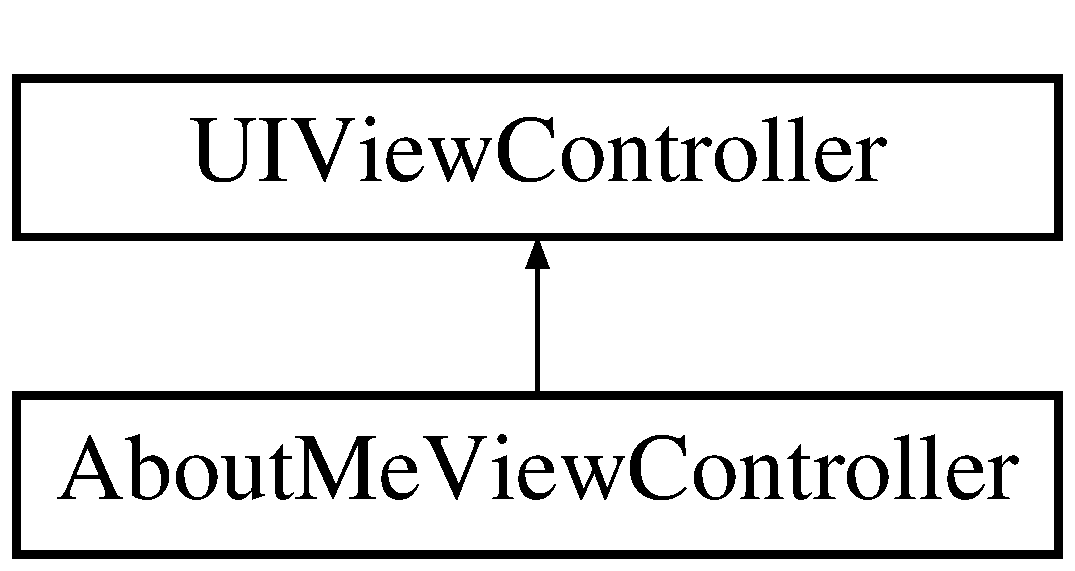
\includegraphics[height=2.000000cm]{interface_about_me_view_controller}
\end{center}
\end{figure}


\subsection{Detailed Description}


Definition at line 11 of file About\+Me\+View\+Controller.\+h.



The documentation for this class was generated from the following file\+:\begin{DoxyCompactItemize}
\item 
/\+Users/\+Jake/\+Google Drive/04\+\_\+\+Projects/\+X\+Code/jacksod.\+a2-\/rev01/jacksod.\+a2/\hyperlink{_about_me_view_controller_8h}{About\+Me\+View\+Controller.\+h}\end{DoxyCompactItemize}

\hypertarget{category_about_me_view_controller_07_08}{\section{About\+Me\+View\+Controller() Category Reference}
\label{category_about_me_view_controller_07_08}\index{About\+Me\+View\+Controller()@{About\+Me\+View\+Controller()}}
}


\subsection{Detailed Description}


Definition at line 11 of file About\+Me\+View\+Controller.\+m.



The documentation for this category was generated from the following file\+:\begin{DoxyCompactItemize}
\item 
/\+Users/\+Jake/\+Google Drive/04\+\_\+\+Projects/\+X\+Code/jacksod.\+a2-\/rev01/jacksod.\+a2/\hyperlink{_about_me_view_controller_8m}{About\+Me\+View\+Controller.\+m}\end{DoxyCompactItemize}

\hypertarget{interface_v_t_k_acknowlegments_view_controller}{\section{V\+T\+K\+Acknowlegments\+View\+Controller Class Reference}
\label{interface_v_t_k_acknowlegments_view_controller}\index{V\+T\+K\+Acknowlegments\+View\+Controller@{V\+T\+K\+Acknowlegments\+View\+Controller}}
}


{\ttfamily \#import $<$V\+T\+K\+Acknowlegments\+View\+Controller.\+h$>$}

Inheritance diagram for V\+T\+K\+Acknowlegments\+View\+Controller\+:\begin{figure}[H]
\begin{center}
\leavevmode
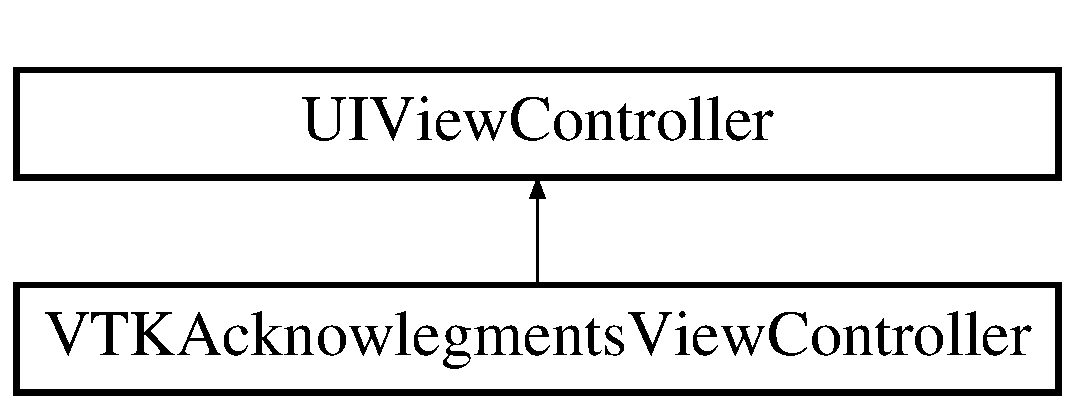
\includegraphics[height=2.000000cm]{interface_v_t_k_acknowlegments_view_controller}
\end{center}
\end{figure}


\subsection{Detailed Description}


Definition at line 11 of file V\+T\+K\+Acknowlegments\+View\+Controller.\+h.



The documentation for this class was generated from the following file\+:\begin{DoxyCompactItemize}
\item 
/\+Users/\+Jake/\+Google Drive/04\+\_\+\+Projects/\+X\+Code/jacksod.\+a2-\/rev01/jacksod.\+a2/\hyperlink{_v_t_k_acknowlegments_view_controller_8h}{V\+T\+K\+Acknowlegments\+View\+Controller.\+h}\end{DoxyCompactItemize}

\hypertarget{category_v_t_k_acknowlegments_view_controller_07_08}{\section{V\+T\+K\+Acknowlegments\+View\+Controller() Category Reference}
\label{category_v_t_k_acknowlegments_view_controller_07_08}\index{V\+T\+K\+Acknowlegments\+View\+Controller()@{V\+T\+K\+Acknowlegments\+View\+Controller()}}
}


\subsection{Detailed Description}


Definition at line 11 of file V\+T\+K\+Acknowlegments\+View\+Controller.\+m.



The documentation for this category was generated from the following file\+:\begin{DoxyCompactItemize}
\item 
/\+Users/\+Jake/\+Google Drive/04\+\_\+\+Projects/\+X\+Code/jacksod.\+a2-\/rev01/jacksod.\+a2/\hyperlink{_v_t_k_acknowlegments_view_controller_8m}{V\+T\+K\+Acknowlegments\+View\+Controller.\+m}\end{DoxyCompactItemize}

\hypertarget{interface_v_t_k_app_delegate}{\section{V\+T\+K\+App\+Delegate Class Reference}
\label{interface_v_t_k_app_delegate}\index{V\+T\+K\+App\+Delegate@{V\+T\+K\+App\+Delegate}}
}


{\ttfamily \#import $<$V\+T\+K\+App\+Delegate.\+h$>$}

Inheritance diagram for V\+T\+K\+App\+Delegate\+:\begin{figure}[H]
\begin{center}
\leavevmode
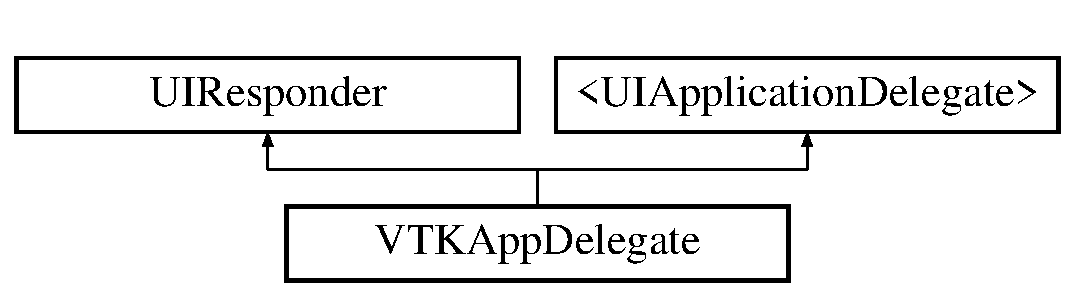
\includegraphics[height=2.000000cm]{interface_v_t_k_app_delegate}
\end{center}
\end{figure}
\subsection*{Properties}
\begin{DoxyCompactItemize}
\item 
U\+I\+Window $\ast$ \hyperlink{interface_v_t_k_app_delegate_a3c0e963db66c6210fda40875bb923e57}{window}
\end{DoxyCompactItemize}


\subsection{Detailed Description}


Definition at line 11 of file V\+T\+K\+App\+Delegate.\+h.



\subsection{Property Documentation}
\hypertarget{interface_v_t_k_app_delegate_a3c0e963db66c6210fda40875bb923e57}{\index{V\+T\+K\+App\+Delegate@{V\+T\+K\+App\+Delegate}!window@{window}}
\index{window@{window}!V\+T\+K\+App\+Delegate@{V\+T\+K\+App\+Delegate}}
\subsubsection[{window}]{\setlength{\rightskip}{0pt plus 5cm}-\/ (U\+I\+Window$\ast$) window\hspace{0.3cm}{\ttfamily [read]}, {\ttfamily [write]}, {\ttfamily [nonatomic]}, {\ttfamily [strong]}}}\label{interface_v_t_k_app_delegate_a3c0e963db66c6210fda40875bb923e57}


Definition at line 13 of file V\+T\+K\+App\+Delegate.\+h.



The documentation for this class was generated from the following file\+:\begin{DoxyCompactItemize}
\item 
/\+Users/\+Jake/\+Google Drive/04\+\_\+\+Projects/\+X\+Code/jacksod.\+a2-\/rev01/jacksod.\+a2/\hyperlink{_v_t_k_app_delegate_8h}{V\+T\+K\+App\+Delegate.\+h}\end{DoxyCompactItemize}

\hypertarget{interface_v_t_k_bitrate_view_controller}{\section{V\+T\+K\+Bitrate\+View\+Controller Class Reference}
\label{interface_v_t_k_bitrate_view_controller}\index{V\+T\+K\+Bitrate\+View\+Controller@{V\+T\+K\+Bitrate\+View\+Controller}}
}


{\ttfamily \#import $<$V\+T\+K\+Bitrate\+View\+Controller.\+h$>$}

Inheritance diagram for V\+T\+K\+Bitrate\+View\+Controller\+:\begin{figure}[H]
\begin{center}
\leavevmode
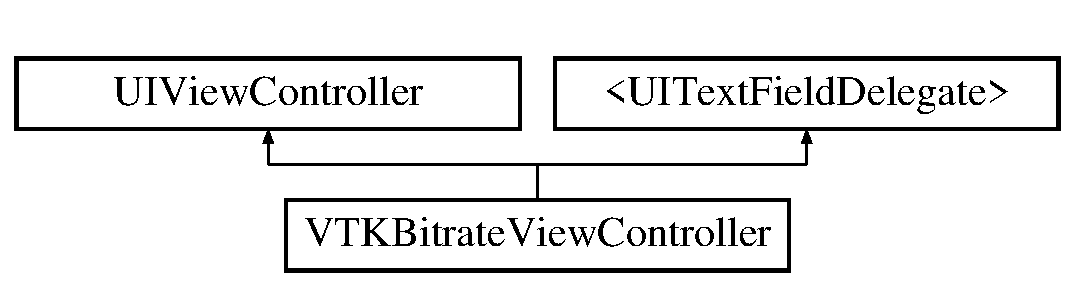
\includegraphics[height=2.000000cm]{interface_v_t_k_bitrate_view_controller}
\end{center}
\end{figure}


\subsection{Detailed Description}


Definition at line 11 of file V\+T\+K\+Bitrate\+View\+Controller.\+h.



The documentation for this class was generated from the following file\+:\begin{DoxyCompactItemize}
\item 
/\+Users/\+Jake/\+Google Drive/04\+\_\+\+Projects/\+X\+Code/jacksod.\+a2-\/rev01/jacksod.\+a2/\hyperlink{_v_t_k_bitrate_view_controller_8h}{V\+T\+K\+Bitrate\+View\+Controller.\+h}\end{DoxyCompactItemize}

\hypertarget{category_v_t_k_bitrate_view_controller_07_08}{\section{V\+T\+K\+Bitrate\+View\+Controller() Category Reference}
\label{category_v_t_k_bitrate_view_controller_07_08}\index{V\+T\+K\+Bitrate\+View\+Controller()@{V\+T\+K\+Bitrate\+View\+Controller()}}
}
\subsection*{Properties}
\begin{DoxyCompactItemize}
\item 
I\+B\+Outlet U\+I\+Text\+Field $\ast$ \hyperlink{category_v_t_k_bitrate_view_controller_07_08_acff0a36c7e5f3051be208ab1ed7851d7}{duration\+Field1}
\item 
I\+B\+Outlet U\+I\+Text\+Field $\ast$ \hyperlink{category_v_t_k_bitrate_view_controller_07_08_a7f677395918cd7188d58e302290c8b81}{bitrate\+Field}
\item 
I\+B\+Outlet U\+I\+Button $\ast$ \hyperlink{category_v_t_k_bitrate_view_controller_07_08_ab6816ccfe5c65c4717d3f5a6414bddd7}{calculate\+File\+Size\+Button}
\item 
I\+B\+Outlet U\+I\+Label $\ast$ \hyperlink{category_v_t_k_bitrate_view_controller_07_08_a659e0d954d37ddedaa9cd9445c701ef3}{file\+Size\+Label}
\item 
I\+B\+Outlet U\+I\+Text\+Field $\ast$ \hyperlink{category_v_t_k_bitrate_view_controller_07_08_a37fa2e54bbf11e3be3e3da9f1b74859f}{duration\+Field2}
\item 
I\+B\+Outlet U\+I\+Text\+Field $\ast$ \hyperlink{category_v_t_k_bitrate_view_controller_07_08_a4cc29123e9b7a76810fbf3c3d842904f}{file\+Size\+Field}
\item 
I\+B\+Outlet U\+I\+Button $\ast$ \hyperlink{category_v_t_k_bitrate_view_controller_07_08_a1e803d315ee50e6c216155e4e1b46cc0}{calculate\+Bitrate\+Button}
\item 
I\+B\+Outlet U\+I\+Label $\ast$ \hyperlink{category_v_t_k_bitrate_view_controller_07_08_a347b6ac7bd388e0492406dfd9baa8585}{bitrate\+Label}
\item 
I\+B\+Outlet U\+I\+Segmented\+Control $\ast$ \hyperlink{category_v_t_k_bitrate_view_controller_07_08_a954b77c570cd18a518d9f46a489c800e}{file\+Size\+Segmented\+Control}
\item 
I\+B\+Outlet U\+I\+Scroll\+View $\ast$ \hyperlink{category_v_t_k_bitrate_view_controller_07_08_abc9eba67908448321fb758b6f1a601f8}{the\+Scroll\+View}
\end{DoxyCompactItemize}


\subsection{Detailed Description}


Definition at line 11 of file V\+T\+K\+Bitrate\+View\+Controller.\+m.



\subsection{Property Documentation}
\hypertarget{category_v_t_k_bitrate_view_controller_07_08_a7f677395918cd7188d58e302290c8b81}{\index{V\+T\+K\+Bitrate\+View\+Controller()@{V\+T\+K\+Bitrate\+View\+Controller()}!bitrate\+Field@{bitrate\+Field}}
\index{bitrate\+Field@{bitrate\+Field}!V\+T\+K\+Bitrate\+View\+Controller()@{V\+T\+K\+Bitrate\+View\+Controller()}}
\subsubsection[{bitrate\+Field}]{\setlength{\rightskip}{0pt plus 5cm}-\/ (I\+B\+Outlet U\+I\+Text\+Field$\ast$) bitrate\+Field\hspace{0.3cm}{\ttfamily [read]}, {\ttfamily [write]}, {\ttfamily [nonatomic]}, {\ttfamily [weak]}}}\label{category_v_t_k_bitrate_view_controller_07_08_a7f677395918cd7188d58e302290c8b81}


Definition at line 13 of file V\+T\+K\+Bitrate\+View\+Controller.\+m.

\hypertarget{category_v_t_k_bitrate_view_controller_07_08_a347b6ac7bd388e0492406dfd9baa8585}{\index{V\+T\+K\+Bitrate\+View\+Controller()@{V\+T\+K\+Bitrate\+View\+Controller()}!bitrate\+Label@{bitrate\+Label}}
\index{bitrate\+Label@{bitrate\+Label}!V\+T\+K\+Bitrate\+View\+Controller()@{V\+T\+K\+Bitrate\+View\+Controller()}}
\subsubsection[{bitrate\+Label}]{\setlength{\rightskip}{0pt plus 5cm}-\/ (I\+B\+Outlet U\+I\+Label$\ast$) bitrate\+Label\hspace{0.3cm}{\ttfamily [read]}, {\ttfamily [write]}, {\ttfamily [nonatomic]}, {\ttfamily [weak]}}}\label{category_v_t_k_bitrate_view_controller_07_08_a347b6ac7bd388e0492406dfd9baa8585}


Definition at line 20 of file V\+T\+K\+Bitrate\+View\+Controller.\+m.

\hypertarget{category_v_t_k_bitrate_view_controller_07_08_a1e803d315ee50e6c216155e4e1b46cc0}{\index{V\+T\+K\+Bitrate\+View\+Controller()@{V\+T\+K\+Bitrate\+View\+Controller()}!calculate\+Bitrate\+Button@{calculate\+Bitrate\+Button}}
\index{calculate\+Bitrate\+Button@{calculate\+Bitrate\+Button}!V\+T\+K\+Bitrate\+View\+Controller()@{V\+T\+K\+Bitrate\+View\+Controller()}}
\subsubsection[{calculate\+Bitrate\+Button}]{\setlength{\rightskip}{0pt plus 5cm}-\/ (I\+B\+Outlet U\+I\+Button$\ast$) calculate\+Bitrate\+Button\hspace{0.3cm}{\ttfamily [read]}, {\ttfamily [write]}, {\ttfamily [nonatomic]}, {\ttfamily [weak]}}}\label{category_v_t_k_bitrate_view_controller_07_08_a1e803d315ee50e6c216155e4e1b46cc0}


Definition at line 19 of file V\+T\+K\+Bitrate\+View\+Controller.\+m.

\hypertarget{category_v_t_k_bitrate_view_controller_07_08_ab6816ccfe5c65c4717d3f5a6414bddd7}{\index{V\+T\+K\+Bitrate\+View\+Controller()@{V\+T\+K\+Bitrate\+View\+Controller()}!calculate\+File\+Size\+Button@{calculate\+File\+Size\+Button}}
\index{calculate\+File\+Size\+Button@{calculate\+File\+Size\+Button}!V\+T\+K\+Bitrate\+View\+Controller()@{V\+T\+K\+Bitrate\+View\+Controller()}}
\subsubsection[{calculate\+File\+Size\+Button}]{\setlength{\rightskip}{0pt plus 5cm}-\/ (I\+B\+Outlet U\+I\+Button$\ast$) calculate\+File\+Size\+Button\hspace{0.3cm}{\ttfamily [read]}, {\ttfamily [write]}, {\ttfamily [nonatomic]}, {\ttfamily [weak]}}}\label{category_v_t_k_bitrate_view_controller_07_08_ab6816ccfe5c65c4717d3f5a6414bddd7}


Definition at line 14 of file V\+T\+K\+Bitrate\+View\+Controller.\+m.

\hypertarget{category_v_t_k_bitrate_view_controller_07_08_acff0a36c7e5f3051be208ab1ed7851d7}{\index{V\+T\+K\+Bitrate\+View\+Controller()@{V\+T\+K\+Bitrate\+View\+Controller()}!duration\+Field1@{duration\+Field1}}
\index{duration\+Field1@{duration\+Field1}!V\+T\+K\+Bitrate\+View\+Controller()@{V\+T\+K\+Bitrate\+View\+Controller()}}
\subsubsection[{duration\+Field1}]{\setlength{\rightskip}{0pt plus 5cm}-\/ (I\+B\+Outlet U\+I\+Text\+Field$\ast$) duration\+Field1\hspace{0.3cm}{\ttfamily [read]}, {\ttfamily [write]}, {\ttfamily [nonatomic]}, {\ttfamily [weak]}}}\label{category_v_t_k_bitrate_view_controller_07_08_acff0a36c7e5f3051be208ab1ed7851d7}


Definition at line 12 of file V\+T\+K\+Bitrate\+View\+Controller.\+m.

\hypertarget{category_v_t_k_bitrate_view_controller_07_08_a37fa2e54bbf11e3be3e3da9f1b74859f}{\index{V\+T\+K\+Bitrate\+View\+Controller()@{V\+T\+K\+Bitrate\+View\+Controller()}!duration\+Field2@{duration\+Field2}}
\index{duration\+Field2@{duration\+Field2}!V\+T\+K\+Bitrate\+View\+Controller()@{V\+T\+K\+Bitrate\+View\+Controller()}}
\subsubsection[{duration\+Field2}]{\setlength{\rightskip}{0pt plus 5cm}-\/ (I\+B\+Outlet U\+I\+Text\+Field$\ast$) duration\+Field2\hspace{0.3cm}{\ttfamily [read]}, {\ttfamily [write]}, {\ttfamily [nonatomic]}, {\ttfamily [weak]}}}\label{category_v_t_k_bitrate_view_controller_07_08_a37fa2e54bbf11e3be3e3da9f1b74859f}


Definition at line 17 of file V\+T\+K\+Bitrate\+View\+Controller.\+m.

\hypertarget{category_v_t_k_bitrate_view_controller_07_08_a4cc29123e9b7a76810fbf3c3d842904f}{\index{V\+T\+K\+Bitrate\+View\+Controller()@{V\+T\+K\+Bitrate\+View\+Controller()}!file\+Size\+Field@{file\+Size\+Field}}
\index{file\+Size\+Field@{file\+Size\+Field}!V\+T\+K\+Bitrate\+View\+Controller()@{V\+T\+K\+Bitrate\+View\+Controller()}}
\subsubsection[{file\+Size\+Field}]{\setlength{\rightskip}{0pt plus 5cm}-\/ (I\+B\+Outlet U\+I\+Text\+Field$\ast$) file\+Size\+Field\hspace{0.3cm}{\ttfamily [read]}, {\ttfamily [write]}, {\ttfamily [nonatomic]}, {\ttfamily [weak]}}}\label{category_v_t_k_bitrate_view_controller_07_08_a4cc29123e9b7a76810fbf3c3d842904f}


Definition at line 18 of file V\+T\+K\+Bitrate\+View\+Controller.\+m.

\hypertarget{category_v_t_k_bitrate_view_controller_07_08_a659e0d954d37ddedaa9cd9445c701ef3}{\index{V\+T\+K\+Bitrate\+View\+Controller()@{V\+T\+K\+Bitrate\+View\+Controller()}!file\+Size\+Label@{file\+Size\+Label}}
\index{file\+Size\+Label@{file\+Size\+Label}!V\+T\+K\+Bitrate\+View\+Controller()@{V\+T\+K\+Bitrate\+View\+Controller()}}
\subsubsection[{file\+Size\+Label}]{\setlength{\rightskip}{0pt plus 5cm}-\/ (I\+B\+Outlet U\+I\+Label$\ast$) file\+Size\+Label\hspace{0.3cm}{\ttfamily [read]}, {\ttfamily [write]}, {\ttfamily [nonatomic]}, {\ttfamily [weak]}}}\label{category_v_t_k_bitrate_view_controller_07_08_a659e0d954d37ddedaa9cd9445c701ef3}


Definition at line 15 of file V\+T\+K\+Bitrate\+View\+Controller.\+m.

\hypertarget{category_v_t_k_bitrate_view_controller_07_08_a954b77c570cd18a518d9f46a489c800e}{\index{V\+T\+K\+Bitrate\+View\+Controller()@{V\+T\+K\+Bitrate\+View\+Controller()}!file\+Size\+Segmented\+Control@{file\+Size\+Segmented\+Control}}
\index{file\+Size\+Segmented\+Control@{file\+Size\+Segmented\+Control}!V\+T\+K\+Bitrate\+View\+Controller()@{V\+T\+K\+Bitrate\+View\+Controller()}}
\subsubsection[{file\+Size\+Segmented\+Control}]{\setlength{\rightskip}{0pt plus 5cm}-\/ (I\+B\+Outlet U\+I\+Segmented\+Control$\ast$) file\+Size\+Segmented\+Control\hspace{0.3cm}{\ttfamily [read]}, {\ttfamily [write]}, {\ttfamily [nonatomic]}, {\ttfamily [weak]}}}\label{category_v_t_k_bitrate_view_controller_07_08_a954b77c570cd18a518d9f46a489c800e}


Definition at line 21 of file V\+T\+K\+Bitrate\+View\+Controller.\+m.

\hypertarget{category_v_t_k_bitrate_view_controller_07_08_abc9eba67908448321fb758b6f1a601f8}{\index{V\+T\+K\+Bitrate\+View\+Controller()@{V\+T\+K\+Bitrate\+View\+Controller()}!the\+Scroll\+View@{the\+Scroll\+View}}
\index{the\+Scroll\+View@{the\+Scroll\+View}!V\+T\+K\+Bitrate\+View\+Controller()@{V\+T\+K\+Bitrate\+View\+Controller()}}
\subsubsection[{the\+Scroll\+View}]{\setlength{\rightskip}{0pt plus 5cm}-\/ (I\+B\+Outlet U\+I\+Scroll\+View$\ast$) the\+Scroll\+View\hspace{0.3cm}{\ttfamily [read]}, {\ttfamily [write]}, {\ttfamily [nonatomic]}, {\ttfamily [weak]}}}\label{category_v_t_k_bitrate_view_controller_07_08_abc9eba67908448321fb758b6f1a601f8}


Definition at line 23 of file V\+T\+K\+Bitrate\+View\+Controller.\+m.



The documentation for this category was generated from the following file\+:\begin{DoxyCompactItemize}
\item 
/\+Users/\+Jake/\+Google Drive/04\+\_\+\+Projects/\+X\+Code/jacksod.\+a2-\/rev01/jacksod.\+a2/\hyperlink{_v_t_k_bitrate_view_controller_8m}{V\+T\+K\+Bitrate\+View\+Controller.\+m}\end{DoxyCompactItemize}

\hypertarget{interface_v_t_k_info_view_controller}{\section{V\+T\+K\+Info\+View\+Controller Class Reference}
\label{interface_v_t_k_info_view_controller}\index{V\+T\+K\+Info\+View\+Controller@{V\+T\+K\+Info\+View\+Controller}}
}


{\ttfamily \#import $<$V\+T\+K\+Info\+View\+Controller.\+h$>$}

Inheritance diagram for V\+T\+K\+Info\+View\+Controller\+:\begin{figure}[H]
\begin{center}
\leavevmode
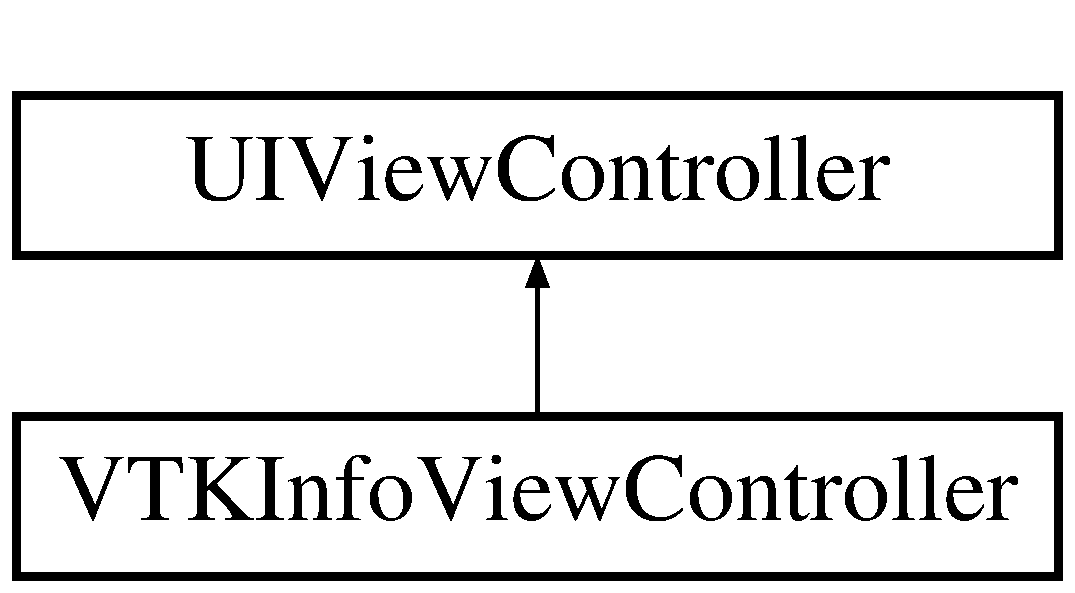
\includegraphics[height=2.000000cm]{interface_v_t_k_info_view_controller}
\end{center}
\end{figure}


\subsection{Detailed Description}


Definition at line 11 of file V\+T\+K\+Info\+View\+Controller.\+h.



The documentation for this class was generated from the following file\+:\begin{DoxyCompactItemize}
\item 
/\+Users/\+Jake/\+Google Drive/04\+\_\+\+Projects/\+X\+Code/jacksod.\+a2-\/rev01/jacksod.\+a2/\hyperlink{_v_t_k_info_view_controller_8h}{V\+T\+K\+Info\+View\+Controller.\+h}\end{DoxyCompactItemize}

\hypertarget{category_v_t_k_info_view_controller_07_08}{\section{V\+T\+K\+Info\+View\+Controller() Category Reference}
\label{category_v_t_k_info_view_controller_07_08}\index{V\+T\+K\+Info\+View\+Controller()@{V\+T\+K\+Info\+View\+Controller()}}
}


\subsection{Detailed Description}


Definition at line 11 of file V\+T\+K\+Info\+View\+Controller.\+m.



The documentation for this category was generated from the following file\+:\begin{DoxyCompactItemize}
\item 
/\+Users/\+Jake/\+Google Drive/04\+\_\+\+Projects/\+X\+Code/jacksod.\+a2-\/rev01/jacksod.\+a2/\hyperlink{_v_t_k_info_view_controller_8m}{V\+T\+K\+Info\+View\+Controller.\+m}\end{DoxyCompactItemize}

\hypertarget{interface_v_t_k_standards_view_controller}{\section{V\+T\+K\+Standards\+View\+Controller Class Reference}
\label{interface_v_t_k_standards_view_controller}\index{V\+T\+K\+Standards\+View\+Controller@{V\+T\+K\+Standards\+View\+Controller}}
}


{\ttfamily \#import $<$V\+T\+K\+Standards\+View\+Controller.\+h$>$}

Inheritance diagram for V\+T\+K\+Standards\+View\+Controller\+:\begin{figure}[H]
\begin{center}
\leavevmode
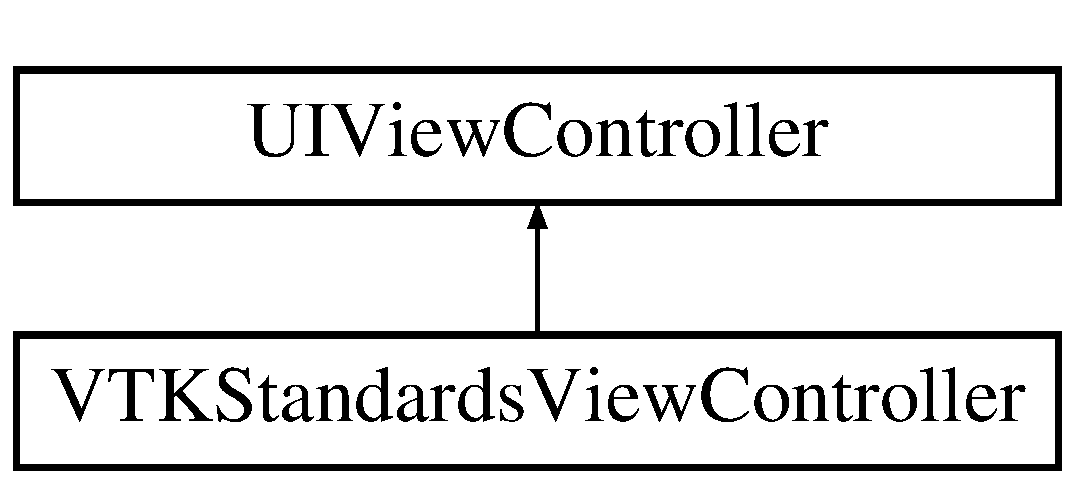
\includegraphics[height=2.000000cm]{interface_v_t_k_standards_view_controller}
\end{center}
\end{figure}
\subsection*{Properties}
\begin{DoxyCompactItemize}
\item 
I\+B\+Outlet U\+I\+Table\+View $\ast$ \hyperlink{interface_v_t_k_standards_view_controller_a80255bab4329e0cc55c67b891340f4e7}{settings\+Table}
\item 
N\+S\+Array $\ast$ \hyperlink{interface_v_t_k_standards_view_controller_a63a0f419f2bf9408c3c5d4f0b19b667d}{settings}
\item 
U\+I\+Refresh\+Control $\ast$ \hyperlink{interface_v_t_k_standards_view_controller_ab4a50d1f06688377ca2759fe6833c8da}{refresh\+Controller}
\end{DoxyCompactItemize}


\subsection{Detailed Description}


Definition at line 12 of file V\+T\+K\+Standards\+View\+Controller.\+h.



\subsection{Property Documentation}
\hypertarget{interface_v_t_k_standards_view_controller_ab4a50d1f06688377ca2759fe6833c8da}{\index{V\+T\+K\+Standards\+View\+Controller@{V\+T\+K\+Standards\+View\+Controller}!refresh\+Controller@{refresh\+Controller}}
\index{refresh\+Controller@{refresh\+Controller}!V\+T\+K\+Standards\+View\+Controller@{V\+T\+K\+Standards\+View\+Controller}}
\subsubsection[{refresh\+Controller}]{\setlength{\rightskip}{0pt plus 5cm}-\/ (U\+I\+Refresh\+Control$\ast$) refresh\+Controller\hspace{0.3cm}{\ttfamily [read]}, {\ttfamily [write]}, {\ttfamily [nonatomic]}, {\ttfamily [assign]}}}\label{interface_v_t_k_standards_view_controller_ab4a50d1f06688377ca2759fe6833c8da}
Our Nitfy refresh\+Controller will allow the Pull-\/to-\/refresh action to take place. 

Definition at line 16 of file V\+T\+K\+Standards\+View\+Controller.\+h.

\hypertarget{interface_v_t_k_standards_view_controller_a63a0f419f2bf9408c3c5d4f0b19b667d}{\index{V\+T\+K\+Standards\+View\+Controller@{V\+T\+K\+Standards\+View\+Controller}!settings@{settings}}
\index{settings@{settings}!V\+T\+K\+Standards\+View\+Controller@{V\+T\+K\+Standards\+View\+Controller}}
\subsubsection[{settings}]{\setlength{\rightskip}{0pt plus 5cm}-\/ (N\+S\+Array$\ast$) settings\hspace{0.3cm}{\ttfamily [read]}, {\ttfamily [write]}, {\ttfamily [nonatomic]}, {\ttfamily [assign]}}}\label{interface_v_t_k_standards_view_controller_a63a0f419f2bf9408c3c5d4f0b19b667d}


Definition at line 15 of file V\+T\+K\+Standards\+View\+Controller.\+h.

\hypertarget{interface_v_t_k_standards_view_controller_a80255bab4329e0cc55c67b891340f4e7}{\index{V\+T\+K\+Standards\+View\+Controller@{V\+T\+K\+Standards\+View\+Controller}!settings\+Table@{settings\+Table}}
\index{settings\+Table@{settings\+Table}!V\+T\+K\+Standards\+View\+Controller@{V\+T\+K\+Standards\+View\+Controller}}
\subsubsection[{settings\+Table}]{\setlength{\rightskip}{0pt plus 5cm}-\/ (I\+B\+Outlet U\+I\+Table\+View$\ast$) settings\+Table\hspace{0.3cm}{\ttfamily [read]}, {\ttfamily [write]}, {\ttfamily [nonatomic]}, {\ttfamily [weak]}}}\label{interface_v_t_k_standards_view_controller_a80255bab4329e0cc55c67b891340f4e7}
The Table the Route will be displayed on. 

Definition at line 14 of file V\+T\+K\+Standards\+View\+Controller.\+h.



The documentation for this class was generated from the following file\+:\begin{DoxyCompactItemize}
\item 
/\+Users/\+Jake/\+Google Drive/04\+\_\+\+Projects/\+X\+Code/jacksod.\+a2-\/rev01/jacksod.\+a2/\hyperlink{_v_t_k_standards_view_controller_8h}{V\+T\+K\+Standards\+View\+Controller.\+h}\end{DoxyCompactItemize}

\hypertarget{category_v_t_k_standards_view_controller_07_08}{\section{V\+T\+K\+Standards\+View\+Controller() Category Reference}
\label{category_v_t_k_standards_view_controller_07_08}\index{V\+T\+K\+Standards\+View\+Controller()@{V\+T\+K\+Standards\+View\+Controller()}}
}
\subsection*{Properties}
\begin{DoxyCompactItemize}
\item 
Vid\+Setting $\ast$ \hyperlink{category_v_t_k_standards_view_controller_07_08_ac3149c7bb132a2a02cd19887536f25d9}{setting\+In\+Focus}
\end{DoxyCompactItemize}


\subsection{Detailed Description}


Definition at line 12 of file V\+T\+K\+Standards\+View\+Controller.\+m.



\subsection{Property Documentation}
\hypertarget{category_v_t_k_standards_view_controller_07_08_ac3149c7bb132a2a02cd19887536f25d9}{\index{V\+T\+K\+Standards\+View\+Controller()@{V\+T\+K\+Standards\+View\+Controller()}!setting\+In\+Focus@{setting\+In\+Focus}}
\index{setting\+In\+Focus@{setting\+In\+Focus}!V\+T\+K\+Standards\+View\+Controller()@{V\+T\+K\+Standards\+View\+Controller()}}
\subsubsection[{setting\+In\+Focus}]{\setlength{\rightskip}{0pt plus 5cm}-\/ (Vid\+Setting$\ast$) setting\+In\+Focus\hspace{0.3cm}{\ttfamily [read]}, {\ttfamily [write]}, {\ttfamily [nonatomic]}, {\ttfamily [strong]}}}\label{category_v_t_k_standards_view_controller_07_08_ac3149c7bb132a2a02cd19887536f25d9}


Definition at line 13 of file V\+T\+K\+Standards\+View\+Controller.\+m.



The documentation for this category was generated from the following file\+:\begin{DoxyCompactItemize}
\item 
/\+Users/\+Jake/\+Google Drive/04\+\_\+\+Projects/\+X\+Code/jacksod.\+a2-\/rev01/jacksod.\+a2/\hyperlink{_v_t_k_standards_view_controller_8m}{V\+T\+K\+Standards\+View\+Controller.\+m}\end{DoxyCompactItemize}

\hypertarget{interface_v_t_k_timecode_controller}{\section{V\+T\+K\+Timecode\+Controller Class Reference}
\label{interface_v_t_k_timecode_controller}\index{V\+T\+K\+Timecode\+Controller@{V\+T\+K\+Timecode\+Controller}}
}


{\ttfamily \#import $<$V\+T\+K\+Timecode\+Controller.\+h$>$}

Inheritance diagram for V\+T\+K\+Timecode\+Controller\+:\begin{figure}[H]
\begin{center}
\leavevmode
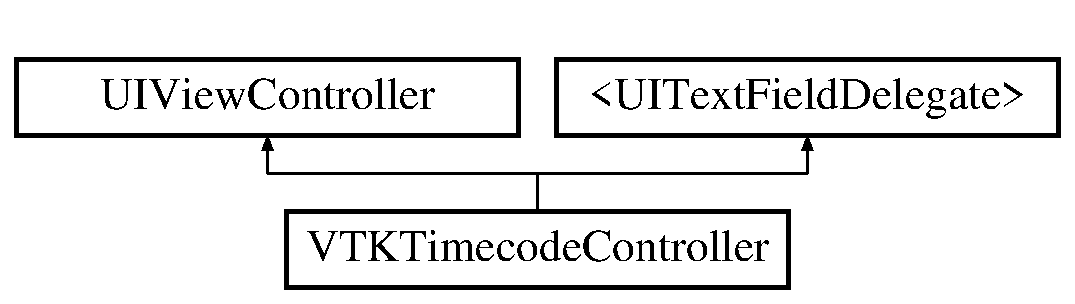
\includegraphics[height=2.000000cm]{interface_v_t_k_timecode_controller}
\end{center}
\end{figure}


\subsection{Detailed Description}


Definition at line 11 of file V\+T\+K\+Timecode\+Controller.\+h.



The documentation for this class was generated from the following file\+:\begin{DoxyCompactItemize}
\item 
/\+Users/\+Jake/\+Google Drive/04\+\_\+\+Projects/\+X\+Code/jacksod.\+a2-\/rev01/jacksod.\+a2/\hyperlink{_v_t_k_timecode_controller_8h}{V\+T\+K\+Timecode\+Controller.\+h}\end{DoxyCompactItemize}

\hypertarget{category_v_t_k_timecode_controller_07_08}{\section{V\+T\+K\+Timecode\+Controller() Category Reference}
\label{category_v_t_k_timecode_controller_07_08}\index{V\+T\+K\+Timecode\+Controller()@{V\+T\+K\+Timecode\+Controller()}}
}
Inheritance diagram for V\+T\+K\+Timecode\+Controller()\+:\begin{figure}[H]
\begin{center}
\leavevmode
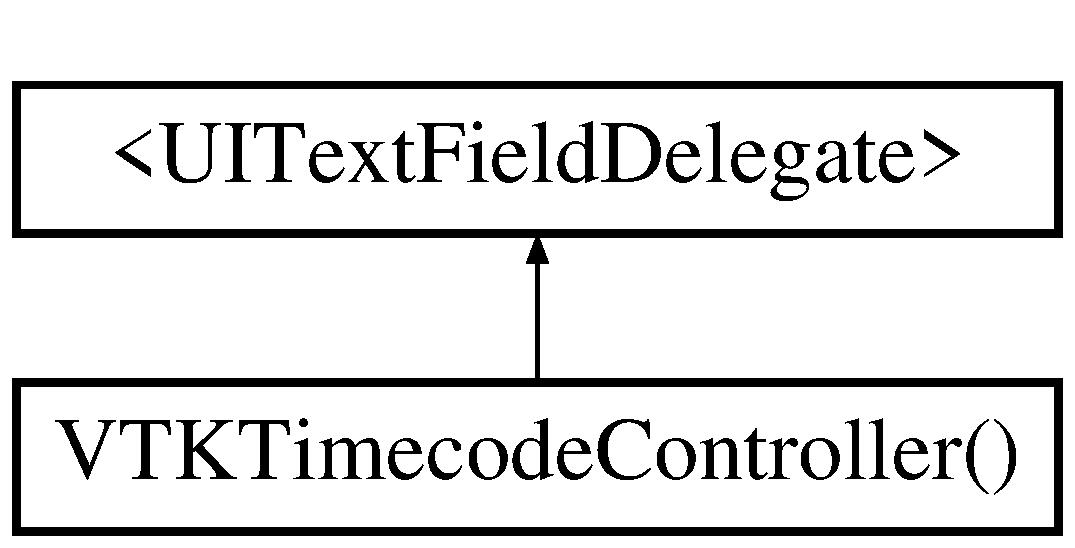
\includegraphics[height=2.000000cm]{category_v_t_k_timecode_controller_07_08}
\end{center}
\end{figure}
\subsection*{Properties}
\begin{DoxyCompactItemize}
\item 
I\+B\+Outlet U\+I\+Text\+Field $\ast$ \hyperlink{category_v_t_k_timecode_controller_07_08_a01e4a2a269595de1df65c643f67ae3c6}{framerate\+Field}
\item 
I\+B\+Outlet U\+I\+Text\+Field $\ast$ \hyperlink{category_v_t_k_timecode_controller_07_08_a24852fbe59ab28cd6a03cd87f63233fa}{time1\+Field}
\item 
I\+B\+Outlet U\+I\+Text\+Field $\ast$ \hyperlink{category_v_t_k_timecode_controller_07_08_a91d07bcd511c8dead712ccbda0ef0ba1}{time2\+Field}
\item 
I\+B\+Outlet U\+I\+Label $\ast$ \hyperlink{category_v_t_k_timecode_controller_07_08_a4e46e7e9fbc90e39d28dcf2e0962c891}{results\+Label}
\end{DoxyCompactItemize}


\subsection{Detailed Description}


Definition at line 11 of file V\+T\+K\+Timecode\+Controller.\+m.



\subsection{Property Documentation}
\hypertarget{category_v_t_k_timecode_controller_07_08_a01e4a2a269595de1df65c643f67ae3c6}{\index{V\+T\+K\+Timecode\+Controller()@{V\+T\+K\+Timecode\+Controller()}!framerate\+Field@{framerate\+Field}}
\index{framerate\+Field@{framerate\+Field}!V\+T\+K\+Timecode\+Controller()@{V\+T\+K\+Timecode\+Controller()}}
\subsubsection[{framerate\+Field}]{\setlength{\rightskip}{0pt plus 5cm}-\/ (I\+B\+Outlet U\+I\+Text\+Field$\ast$) framerate\+Field\hspace{0.3cm}{\ttfamily [read]}, {\ttfamily [write]}, {\ttfamily [nonatomic]}, {\ttfamily [weak]}}}\label{category_v_t_k_timecode_controller_07_08_a01e4a2a269595de1df65c643f67ae3c6}


Definition at line 12 of file V\+T\+K\+Timecode\+Controller.\+m.

\hypertarget{category_v_t_k_timecode_controller_07_08_a4e46e7e9fbc90e39d28dcf2e0962c891}{\index{V\+T\+K\+Timecode\+Controller()@{V\+T\+K\+Timecode\+Controller()}!results\+Label@{results\+Label}}
\index{results\+Label@{results\+Label}!V\+T\+K\+Timecode\+Controller()@{V\+T\+K\+Timecode\+Controller()}}
\subsubsection[{results\+Label}]{\setlength{\rightskip}{0pt plus 5cm}-\/ (I\+B\+Outlet U\+I\+Label$\ast$) results\+Label\hspace{0.3cm}{\ttfamily [read]}, {\ttfamily [write]}, {\ttfamily [nonatomic]}, {\ttfamily [weak]}}}\label{category_v_t_k_timecode_controller_07_08_a4e46e7e9fbc90e39d28dcf2e0962c891}


Definition at line 15 of file V\+T\+K\+Timecode\+Controller.\+m.

\hypertarget{category_v_t_k_timecode_controller_07_08_a24852fbe59ab28cd6a03cd87f63233fa}{\index{V\+T\+K\+Timecode\+Controller()@{V\+T\+K\+Timecode\+Controller()}!time1\+Field@{time1\+Field}}
\index{time1\+Field@{time1\+Field}!V\+T\+K\+Timecode\+Controller()@{V\+T\+K\+Timecode\+Controller()}}
\subsubsection[{time1\+Field}]{\setlength{\rightskip}{0pt plus 5cm}-\/ (I\+B\+Outlet U\+I\+Text\+Field$\ast$) time1\+Field\hspace{0.3cm}{\ttfamily [read]}, {\ttfamily [write]}, {\ttfamily [nonatomic]}, {\ttfamily [weak]}}}\label{category_v_t_k_timecode_controller_07_08_a24852fbe59ab28cd6a03cd87f63233fa}


Definition at line 13 of file V\+T\+K\+Timecode\+Controller.\+m.

\hypertarget{category_v_t_k_timecode_controller_07_08_a91d07bcd511c8dead712ccbda0ef0ba1}{\index{V\+T\+K\+Timecode\+Controller()@{V\+T\+K\+Timecode\+Controller()}!time2\+Field@{time2\+Field}}
\index{time2\+Field@{time2\+Field}!V\+T\+K\+Timecode\+Controller()@{V\+T\+K\+Timecode\+Controller()}}
\subsubsection[{time2\+Field}]{\setlength{\rightskip}{0pt plus 5cm}-\/ (I\+B\+Outlet U\+I\+Text\+Field$\ast$) time2\+Field\hspace{0.3cm}{\ttfamily [read]}, {\ttfamily [write]}, {\ttfamily [nonatomic]}, {\ttfamily [weak]}}}\label{category_v_t_k_timecode_controller_07_08_a91d07bcd511c8dead712ccbda0ef0ba1}


Definition at line 14 of file V\+T\+K\+Timecode\+Controller.\+m.



The documentation for this category was generated from the following file\+:\begin{DoxyCompactItemize}
\item 
/\+Users/\+Jake/\+Google Drive/04\+\_\+\+Projects/\+X\+Code/jacksod.\+a2-\/rev01/jacksod.\+a2/\hyperlink{_v_t_k_timecode_controller_8m}{V\+T\+K\+Timecode\+Controller.\+m}\end{DoxyCompactItemize}

\hypertarget{interface_v_t_k_view_controller}{\section{V\+T\+K\+View\+Controller Class Reference}
\label{interface_v_t_k_view_controller}\index{V\+T\+K\+View\+Controller@{V\+T\+K\+View\+Controller}}
}


{\ttfamily \#import $<$V\+T\+K\+View\+Controller.\+h$>$}

Inheritance diagram for V\+T\+K\+View\+Controller\+:\begin{figure}[H]
\begin{center}
\leavevmode
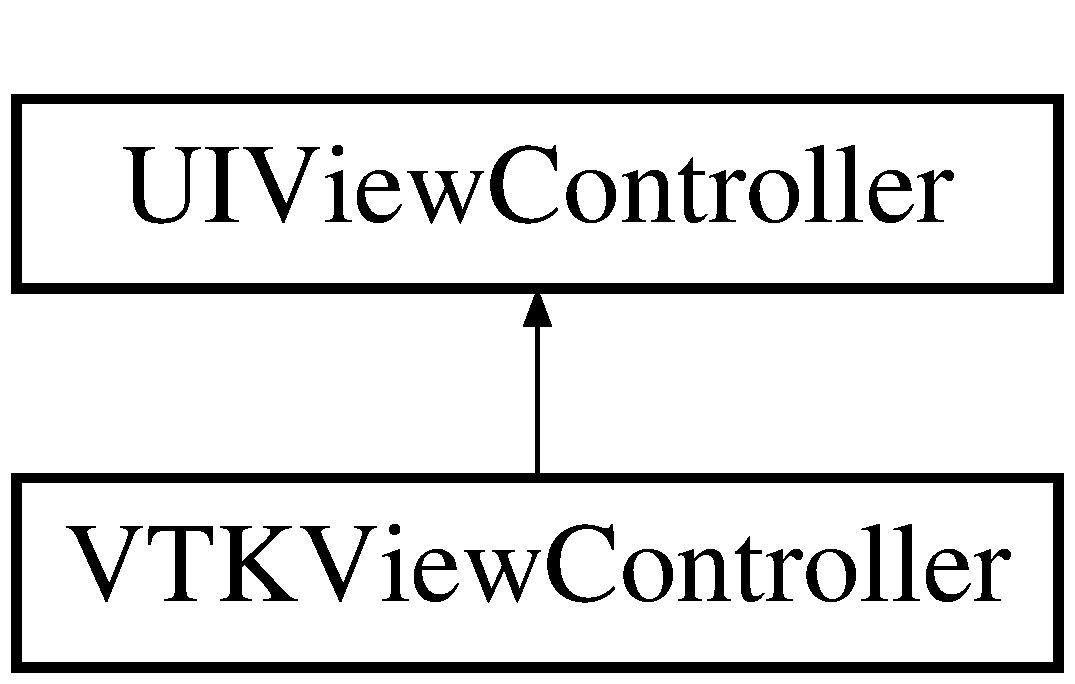
\includegraphics[height=2.000000cm]{interface_v_t_k_view_controller}
\end{center}
\end{figure}


\subsection{Detailed Description}


Definition at line 11 of file V\+T\+K\+View\+Controller.\+h.



The documentation for this class was generated from the following file\+:\begin{DoxyCompactItemize}
\item 
/\+Users/\+Jake/\+Google Drive/04\+\_\+\+Projects/\+X\+Code/jacksod.\+a2-\/rev01/jacksod.\+a2/\hyperlink{_v_t_k_view_controller_8h}{V\+T\+K\+View\+Controller.\+h}\end{DoxyCompactItemize}

\hypertarget{category_v_t_k_view_controller_07_08}{\section{V\+T\+K\+View\+Controller() Category Reference}
\label{category_v_t_k_view_controller_07_08}\index{V\+T\+K\+View\+Controller()@{V\+T\+K\+View\+Controller()}}
}


\subsection{Detailed Description}


Definition at line 11 of file V\+T\+K\+View\+Controller.\+m.



The documentation for this category was generated from the following file\+:\begin{DoxyCompactItemize}
\item 
/\+Users/\+Jake/\+Google Drive/04\+\_\+\+Projects/\+X\+Code/jacksod.\+a2-\/rev01/jacksod.\+a2/\hyperlink{_v_t_k_view_controller_8m}{V\+T\+K\+View\+Controller.\+m}\end{DoxyCompactItemize}

\chapter{File Documentation}
\hypertarget{_about_me_view_controller_8h}{\section{/\+Users/\+Jake/\+Google Drive/04\+\_\+\+Projects/\+X\+Code/jacksod.a2-\/rev01/jacksod.a2/\+About\+Me\+View\+Controller.h File Reference}
\label{_about_me_view_controller_8h}\index{/\+Users/\+Jake/\+Google Drive/04\+\_\+\+Projects/\+X\+Code/jacksod.\+a2-\/rev01/jacksod.\+a2/\+About\+Me\+View\+Controller.\+h@{/\+Users/\+Jake/\+Google Drive/04\+\_\+\+Projects/\+X\+Code/jacksod.\+a2-\/rev01/jacksod.\+a2/\+About\+Me\+View\+Controller.\+h}}
}
{\ttfamily \#import $<$U\+I\+Kit/\+U\+I\+Kit.\+h$>$}\\*
\subsection*{Classes}
\begin{DoxyCompactItemize}
\item 
class \hyperlink{interface_about_me_view_controller}{About\+Me\+View\+Controller}
\end{DoxyCompactItemize}

\hypertarget{_about_me_view_controller_8m}{\section{/\+Users/\+Jake/\+Google Drive/04\+\_\+\+Projects/\+X\+Code/jacksod.a2-\/rev01/jacksod.a2/\+About\+Me\+View\+Controller.m File Reference}
\label{_about_me_view_controller_8m}\index{/\+Users/\+Jake/\+Google Drive/04\+\_\+\+Projects/\+X\+Code/jacksod.\+a2-\/rev01/jacksod.\+a2/\+About\+Me\+View\+Controller.\+m@{/\+Users/\+Jake/\+Google Drive/04\+\_\+\+Projects/\+X\+Code/jacksod.\+a2-\/rev01/jacksod.\+a2/\+About\+Me\+View\+Controller.\+m}}
}
{\ttfamily \#import \char`\"{}About\+Me\+View\+Controller.\+h\char`\"{}}\\*

\hypertarget{_codec_8m}{\section{/\+Users/\+Jake/\+Google Drive/04\+\_\+\+Projects/\+X\+Code/jacksod.a2-\/rev01/jacksod.a2/\+Codec.m File Reference}
\label{_codec_8m}\index{/\+Users/\+Jake/\+Google Drive/04\+\_\+\+Projects/\+X\+Code/jacksod.\+a2-\/rev01/jacksod.\+a2/\+Codec.\+m@{/\+Users/\+Jake/\+Google Drive/04\+\_\+\+Projects/\+X\+Code/jacksod.\+a2-\/rev01/jacksod.\+a2/\+Codec.\+m}}
}
{\ttfamily \#import \char`\"{}Codec.\+h\char`\"{}}\\*

\hypertarget{database_8h}{\section{/\+Users/\+Jake/\+Google Drive/04\+\_\+\+Projects/\+X\+Code/jacksod.a2-\/rev01/jacksod.a2/database.h File Reference}
\label{database_8h}\index{/\+Users/\+Jake/\+Google Drive/04\+\_\+\+Projects/\+X\+Code/jacksod.\+a2-\/rev01/jacksod.\+a2/database.\+h@{/\+Users/\+Jake/\+Google Drive/04\+\_\+\+Projects/\+X\+Code/jacksod.\+a2-\/rev01/jacksod.\+a2/database.\+h}}
}
{\ttfamily \#import \char`\"{}Vid\+Setting.\+h\char`\"{}}\\*
{\ttfamily \#import \char`\"{}sqlite3.\+h\char`\"{}}\\*
{\ttfamily \#import \char`\"{}Codec.\+h\char`\"{}}\\*

\hypertarget{database_8m}{\section{/\+Users/\+Jake/\+Google Drive/04\+\_\+\+Projects/\+X\+Code/jacksod.a2-\/rev01/jacksod.a2/database.m File Reference}
\label{database_8m}\index{/\+Users/\+Jake/\+Google Drive/04\+\_\+\+Projects/\+X\+Code/jacksod.\+a2-\/rev01/jacksod.\+a2/database.\+m@{/\+Users/\+Jake/\+Google Drive/04\+\_\+\+Projects/\+X\+Code/jacksod.\+a2-\/rev01/jacksod.\+a2/database.\+m}}
}
{\ttfamily \#import \char`\"{}Database.\+h\char`\"{}}\\*

\hypertarget{main_8m}{\section{/\+Users/\+Jake/\+Google Drive/04\+\_\+\+Projects/\+X\+Code/jacksod.a2-\/rev01/jacksod.a2/main.m File Reference}
\label{main_8m}\index{/\+Users/\+Jake/\+Google Drive/04\+\_\+\+Projects/\+X\+Code/jacksod.\+a2-\/rev01/jacksod.\+a2/main.\+m@{/\+Users/\+Jake/\+Google Drive/04\+\_\+\+Projects/\+X\+Code/jacksod.\+a2-\/rev01/jacksod.\+a2/main.\+m}}
}
{\ttfamily \#import $<$U\+I\+Kit/\+U\+I\+Kit.\+h$>$}\\*
{\ttfamily \#import \char`\"{}V\+T\+K\+App\+Delegate.\+h\char`\"{}}\\*
\subsection*{Functions}
\begin{DoxyCompactItemize}
\item 
int \hyperlink{main_8m_a0ddf1224851353fc92bfbff6f499fa97}{main} (int argc, char $\ast$argv\mbox{[}$\,$\mbox{]})
\end{DoxyCompactItemize}


\subsection{Function Documentation}
\hypertarget{main_8m_a0ddf1224851353fc92bfbff6f499fa97}{\index{main.\+m@{main.\+m}!main@{main}}
\index{main@{main}!main.\+m@{main.\+m}}
\subsubsection[{main}]{\setlength{\rightskip}{0pt plus 5cm}int main (
\begin{DoxyParamCaption}
\item[{int}]{argc, }
\item[{char $\ast$}]{argv\mbox{[}$\,$\mbox{]}}
\end{DoxyParamCaption}
)}}\label{main_8m_a0ddf1224851353fc92bfbff6f499fa97}


Definition at line 13 of file main.\+m.


\hypertarget{_vid_setting_8h}{\section{/\+Users/\+Jake/\+Google Drive/04\+\_\+\+Projects/\+X\+Code/jacksod.a2-\/rev01/jacksod.a2/\+Vid\+Setting.h File Reference}
\label{_vid_setting_8h}\index{/\+Users/\+Jake/\+Google Drive/04\+\_\+\+Projects/\+X\+Code/jacksod.\+a2-\/rev01/jacksod.\+a2/\+Vid\+Setting.\+h@{/\+Users/\+Jake/\+Google Drive/04\+\_\+\+Projects/\+X\+Code/jacksod.\+a2-\/rev01/jacksod.\+a2/\+Vid\+Setting.\+h}}
}
{\ttfamily \#import $<$Foundation/\+Foundation.\+h$>$}\\*

\hypertarget{_vid_setting_8m}{\section{/\+Users/\+Jake/\+Google Drive/04\+\_\+\+Projects/\+X\+Code/jacksod.a2-\/rev01/jacksod.a2/\+Vid\+Setting.m File Reference}
\label{_vid_setting_8m}\index{/\+Users/\+Jake/\+Google Drive/04\+\_\+\+Projects/\+X\+Code/jacksod.\+a2-\/rev01/jacksod.\+a2/\+Vid\+Setting.\+m@{/\+Users/\+Jake/\+Google Drive/04\+\_\+\+Projects/\+X\+Code/jacksod.\+a2-\/rev01/jacksod.\+a2/\+Vid\+Setting.\+m}}
}
{\ttfamily \#import \char`\"{}Vid\+Setting.\+h\char`\"{}}\\*

\hypertarget{_v_t_k_acknowlegments_view_controller_8h}{\section{/\+Users/\+Jake/\+Google Drive/04\+\_\+\+Projects/\+X\+Code/jacksod.a2-\/rev01/jacksod.a2/\+V\+T\+K\+Acknowlegments\+View\+Controller.h File Reference}
\label{_v_t_k_acknowlegments_view_controller_8h}\index{/\+Users/\+Jake/\+Google Drive/04\+\_\+\+Projects/\+X\+Code/jacksod.\+a2-\/rev01/jacksod.\+a2/\+V\+T\+K\+Acknowlegments\+View\+Controller.\+h@{/\+Users/\+Jake/\+Google Drive/04\+\_\+\+Projects/\+X\+Code/jacksod.\+a2-\/rev01/jacksod.\+a2/\+V\+T\+K\+Acknowlegments\+View\+Controller.\+h}}
}
{\ttfamily \#import $<$U\+I\+Kit/\+U\+I\+Kit.\+h$>$}\\*
\subsection*{Classes}
\begin{DoxyCompactItemize}
\item 
class \hyperlink{interface_v_t_k_acknowlegments_view_controller}{V\+T\+K\+Acknowlegments\+View\+Controller}
\end{DoxyCompactItemize}

\hypertarget{_v_t_k_acknowlegments_view_controller_8m}{\section{/\+Users/\+Jake/\+Google Drive/04\+\_\+\+Projects/\+X\+Code/jacksod.a2-\/rev01/jacksod.a2/\+V\+T\+K\+Acknowlegments\+View\+Controller.m File Reference}
\label{_v_t_k_acknowlegments_view_controller_8m}\index{/\+Users/\+Jake/\+Google Drive/04\+\_\+\+Projects/\+X\+Code/jacksod.\+a2-\/rev01/jacksod.\+a2/\+V\+T\+K\+Acknowlegments\+View\+Controller.\+m@{/\+Users/\+Jake/\+Google Drive/04\+\_\+\+Projects/\+X\+Code/jacksod.\+a2-\/rev01/jacksod.\+a2/\+V\+T\+K\+Acknowlegments\+View\+Controller.\+m}}
}
{\ttfamily \#import \char`\"{}V\+T\+K\+Acknowlegments\+View\+Controller.\+h\char`\"{}}\\*

\hypertarget{_v_t_k_add_setting_view_controller_8h}{\section{/\+Users/\+Jake/\+Google Drive/04\+\_\+\+Projects/\+X\+Code/jacksod.a2-\/rev01/jacksod.a2/\+V\+T\+K\+Add\+Setting\+View\+Controller.h File Reference}
\label{_v_t_k_add_setting_view_controller_8h}\index{/\+Users/\+Jake/\+Google Drive/04\+\_\+\+Projects/\+X\+Code/jacksod.\+a2-\/rev01/jacksod.\+a2/\+V\+T\+K\+Add\+Setting\+View\+Controller.\+h@{/\+Users/\+Jake/\+Google Drive/04\+\_\+\+Projects/\+X\+Code/jacksod.\+a2-\/rev01/jacksod.\+a2/\+V\+T\+K\+Add\+Setting\+View\+Controller.\+h}}
}
{\ttfamily \#import \char`\"{}database.\+h\char`\"{}}\\*

\hypertarget{_v_t_k_add_setting_view_controller_8m}{\section{/\+Users/\+Jake/\+Google Drive/04\+\_\+\+Projects/\+X\+Code/jacksod.a2-\/rev01/jacksod.a2/\+V\+T\+K\+Add\+Setting\+View\+Controller.m File Reference}
\label{_v_t_k_add_setting_view_controller_8m}\index{/\+Users/\+Jake/\+Google Drive/04\+\_\+\+Projects/\+X\+Code/jacksod.\+a2-\/rev01/jacksod.\+a2/\+V\+T\+K\+Add\+Setting\+View\+Controller.\+m@{/\+Users/\+Jake/\+Google Drive/04\+\_\+\+Projects/\+X\+Code/jacksod.\+a2-\/rev01/jacksod.\+a2/\+V\+T\+K\+Add\+Setting\+View\+Controller.\+m}}
}
{\ttfamily \#import $<$Foundation/\+Foundation.\+h$>$}\\*
{\ttfamily \#import \char`\"{}V\+T\+K\+Add\+Setting\+View\+Controller.\+h\char`\"{}}\\*

\hypertarget{_v_t_k_app_delegate_8h}{\section{/\+Users/\+Jake/\+Google Drive/04\+\_\+\+Projects/\+X\+Code/jacksod.a2-\/rev01/jacksod.a2/\+V\+T\+K\+App\+Delegate.h File Reference}
\label{_v_t_k_app_delegate_8h}\index{/\+Users/\+Jake/\+Google Drive/04\+\_\+\+Projects/\+X\+Code/jacksod.\+a2-\/rev01/jacksod.\+a2/\+V\+T\+K\+App\+Delegate.\+h@{/\+Users/\+Jake/\+Google Drive/04\+\_\+\+Projects/\+X\+Code/jacksod.\+a2-\/rev01/jacksod.\+a2/\+V\+T\+K\+App\+Delegate.\+h}}
}
{\ttfamily \#import $<$U\+I\+Kit/\+U\+I\+Kit.\+h$>$}\\*
\subsection*{Classes}
\begin{DoxyCompactItemize}
\item 
class \hyperlink{interface_v_t_k_app_delegate}{V\+T\+K\+App\+Delegate}
\end{DoxyCompactItemize}

\hypertarget{_v_t_k_app_delegate_8m}{\section{/\+Users/\+Jake/\+Google Drive/04\+\_\+\+Projects/\+X\+Code/jacksod.a2-\/rev01/jacksod.a2/\+V\+T\+K\+App\+Delegate.m File Reference}
\label{_v_t_k_app_delegate_8m}\index{/\+Users/\+Jake/\+Google Drive/04\+\_\+\+Projects/\+X\+Code/jacksod.\+a2-\/rev01/jacksod.\+a2/\+V\+T\+K\+App\+Delegate.\+m@{/\+Users/\+Jake/\+Google Drive/04\+\_\+\+Projects/\+X\+Code/jacksod.\+a2-\/rev01/jacksod.\+a2/\+V\+T\+K\+App\+Delegate.\+m}}
}
{\ttfamily \#import \char`\"{}V\+T\+K\+App\+Delegate.\+h\char`\"{}}\\*

\hypertarget{_v_t_k_bitrate_view_controller_8h}{\section{/\+Users/\+Jake/\+Google Drive/04\+\_\+\+Projects/\+X\+Code/jacksod.a2-\/rev01/jacksod.a2/\+V\+T\+K\+Bitrate\+View\+Controller.h File Reference}
\label{_v_t_k_bitrate_view_controller_8h}\index{/\+Users/\+Jake/\+Google Drive/04\+\_\+\+Projects/\+X\+Code/jacksod.\+a2-\/rev01/jacksod.\+a2/\+V\+T\+K\+Bitrate\+View\+Controller.\+h@{/\+Users/\+Jake/\+Google Drive/04\+\_\+\+Projects/\+X\+Code/jacksod.\+a2-\/rev01/jacksod.\+a2/\+V\+T\+K\+Bitrate\+View\+Controller.\+h}}
}
{\ttfamily \#import $<$U\+I\+Kit/\+U\+I\+Kit.\+h$>$}\\*
\subsection*{Classes}
\begin{DoxyCompactItemize}
\item 
class \hyperlink{interface_v_t_k_bitrate_view_controller}{V\+T\+K\+Bitrate\+View\+Controller}
\end{DoxyCompactItemize}

\hypertarget{_v_t_k_bitrate_view_controller_8m}{\section{/\+Users/\+Jake/\+Google Drive/04\+\_\+\+Projects/\+X\+Code/jacksod.a2-\/rev01/jacksod.a2/\+V\+T\+K\+Bitrate\+View\+Controller.m File Reference}
\label{_v_t_k_bitrate_view_controller_8m}\index{/\+Users/\+Jake/\+Google Drive/04\+\_\+\+Projects/\+X\+Code/jacksod.\+a2-\/rev01/jacksod.\+a2/\+V\+T\+K\+Bitrate\+View\+Controller.\+m@{/\+Users/\+Jake/\+Google Drive/04\+\_\+\+Projects/\+X\+Code/jacksod.\+a2-\/rev01/jacksod.\+a2/\+V\+T\+K\+Bitrate\+View\+Controller.\+m}}
}
{\ttfamily \#import \char`\"{}V\+T\+K\+Bitrate\+View\+Controller.\+h\char`\"{}}\\*

\hypertarget{_v_t_k_codec_detail_view_controller_8h}{\section{/\+Users/\+Jake/\+Google Drive/04\+\_\+\+Projects/\+X\+Code/jacksod.a2-\/rev01/jacksod.a2/\+V\+T\+K\+Codec\+Detail\+View\+Controller.h File Reference}
\label{_v_t_k_codec_detail_view_controller_8h}\index{/\+Users/\+Jake/\+Google Drive/04\+\_\+\+Projects/\+X\+Code/jacksod.\+a2-\/rev01/jacksod.\+a2/\+V\+T\+K\+Codec\+Detail\+View\+Controller.\+h@{/\+Users/\+Jake/\+Google Drive/04\+\_\+\+Projects/\+X\+Code/jacksod.\+a2-\/rev01/jacksod.\+a2/\+V\+T\+K\+Codec\+Detail\+View\+Controller.\+h}}
}
{\ttfamily \#import $<$Foundation/\+Foundation.\+h$>$}\\*
{\ttfamily \#import \char`\"{}database.\+h\char`\"{}}\\*
{\ttfamily \#import $<$U\+I\+Kit/\+U\+I\+Kit.\+h$>$}\\*

\hypertarget{_v_t_k_codec_detail_view_controller_8m}{\section{/\+Users/\+Jake/\+Google Drive/04\+\_\+\+Projects/\+X\+Code/jacksod.a2-\/rev01/jacksod.a2/\+V\+T\+K\+Codec\+Detail\+View\+Controller.m File Reference}
\label{_v_t_k_codec_detail_view_controller_8m}\index{/\+Users/\+Jake/\+Google Drive/04\+\_\+\+Projects/\+X\+Code/jacksod.\+a2-\/rev01/jacksod.\+a2/\+V\+T\+K\+Codec\+Detail\+View\+Controller.\+m@{/\+Users/\+Jake/\+Google Drive/04\+\_\+\+Projects/\+X\+Code/jacksod.\+a2-\/rev01/jacksod.\+a2/\+V\+T\+K\+Codec\+Detail\+View\+Controller.\+m}}
}
{\ttfamily \#import \char`\"{}V\+T\+K\+Codec\+Detail\+View\+Controller.\+h\char`\"{}}\\*
{\ttfamily \#import \char`\"{}V\+T\+K\+Edit\+Setting\+View\+Controller.\+h\char`\"{}}\\*

\hypertarget{_v_t_k_edit_setting_view_controller_8h}{\section{/\+Users/\+Jake/\+Google Drive/04\+\_\+\+Projects/\+X\+Code/jacksod.a2-\/rev01/jacksod.a2/\+V\+T\+K\+Edit\+Setting\+View\+Controller.h File Reference}
\label{_v_t_k_edit_setting_view_controller_8h}\index{/\+Users/\+Jake/\+Google Drive/04\+\_\+\+Projects/\+X\+Code/jacksod.\+a2-\/rev01/jacksod.\+a2/\+V\+T\+K\+Edit\+Setting\+View\+Controller.\+h@{/\+Users/\+Jake/\+Google Drive/04\+\_\+\+Projects/\+X\+Code/jacksod.\+a2-\/rev01/jacksod.\+a2/\+V\+T\+K\+Edit\+Setting\+View\+Controller.\+h}}
}
{\ttfamily \#import $<$U\+I\+Kit/\+U\+I\+Kit.\+h$>$}\\*
{\ttfamily \#import \char`\"{}database.\+h\char`\"{}}\\*
{\ttfamily \#import $<$Foundation/\+Foundation.\+h$>$}\\*

\hypertarget{_v_t_k_edit_setting_view_controller_8m}{\section{/\+Users/\+Jake/\+Google Drive/04\+\_\+\+Projects/\+X\+Code/jacksod.a2-\/rev01/jacksod.a2/\+V\+T\+K\+Edit\+Setting\+View\+Controller.m File Reference}
\label{_v_t_k_edit_setting_view_controller_8m}\index{/\+Users/\+Jake/\+Google Drive/04\+\_\+\+Projects/\+X\+Code/jacksod.\+a2-\/rev01/jacksod.\+a2/\+V\+T\+K\+Edit\+Setting\+View\+Controller.\+m@{/\+Users/\+Jake/\+Google Drive/04\+\_\+\+Projects/\+X\+Code/jacksod.\+a2-\/rev01/jacksod.\+a2/\+V\+T\+K\+Edit\+Setting\+View\+Controller.\+m}}
}
{\ttfamily \#import \char`\"{}V\+T\+K\+Edit\+Setting\+View\+Controller.\+h\char`\"{}}\\*

\hypertarget{_v_t_k_info_view_controller_8h}{\section{/\+Users/\+Jake/\+Google Drive/04\+\_\+\+Projects/\+X\+Code/jacksod.a2-\/rev01/jacksod.a2/\+V\+T\+K\+Info\+View\+Controller.h File Reference}
\label{_v_t_k_info_view_controller_8h}\index{/\+Users/\+Jake/\+Google Drive/04\+\_\+\+Projects/\+X\+Code/jacksod.\+a2-\/rev01/jacksod.\+a2/\+V\+T\+K\+Info\+View\+Controller.\+h@{/\+Users/\+Jake/\+Google Drive/04\+\_\+\+Projects/\+X\+Code/jacksod.\+a2-\/rev01/jacksod.\+a2/\+V\+T\+K\+Info\+View\+Controller.\+h}}
}
{\ttfamily \#import $<$U\+I\+Kit/\+U\+I\+Kit.\+h$>$}\\*
\subsection*{Classes}
\begin{DoxyCompactItemize}
\item 
class \hyperlink{interface_v_t_k_info_view_controller}{V\+T\+K\+Info\+View\+Controller}
\end{DoxyCompactItemize}

\hypertarget{_v_t_k_info_view_controller_8m}{\section{/\+Users/\+Jake/\+Google Drive/04\+\_\+\+Projects/\+X\+Code/jacksod.a2-\/rev01/jacksod.a2/\+V\+T\+K\+Info\+View\+Controller.m File Reference}
\label{_v_t_k_info_view_controller_8m}\index{/\+Users/\+Jake/\+Google Drive/04\+\_\+\+Projects/\+X\+Code/jacksod.\+a2-\/rev01/jacksod.\+a2/\+V\+T\+K\+Info\+View\+Controller.\+m@{/\+Users/\+Jake/\+Google Drive/04\+\_\+\+Projects/\+X\+Code/jacksod.\+a2-\/rev01/jacksod.\+a2/\+V\+T\+K\+Info\+View\+Controller.\+m}}
}
{\ttfamily \#import \char`\"{}V\+T\+K\+Info\+View\+Controller.\+h\char`\"{}}\\*

\hypertarget{_v_t_k_standards_view_controller_8h}{\section{/\+Users/\+Jake/\+Google Drive/04\+\_\+\+Projects/\+X\+Code/jacksod.a2-\/rev01/jacksod.a2/\+V\+T\+K\+Standards\+View\+Controller.h File Reference}
\label{_v_t_k_standards_view_controller_8h}\index{/\+Users/\+Jake/\+Google Drive/04\+\_\+\+Projects/\+X\+Code/jacksod.\+a2-\/rev01/jacksod.\+a2/\+V\+T\+K\+Standards\+View\+Controller.\+h@{/\+Users/\+Jake/\+Google Drive/04\+\_\+\+Projects/\+X\+Code/jacksod.\+a2-\/rev01/jacksod.\+a2/\+V\+T\+K\+Standards\+View\+Controller.\+h}}
}
{\ttfamily \#import $<$U\+I\+Kit/\+U\+I\+Kit.\+h$>$}\\*
{\ttfamily \#import \char`\"{}database.\+h\char`\"{}}\\*
\subsection*{Classes}
\begin{DoxyCompactItemize}
\item 
class \hyperlink{interface_v_t_k_standards_view_controller}{V\+T\+K\+Standards\+View\+Controller}
\end{DoxyCompactItemize}

\hypertarget{_v_t_k_standards_view_controller_8m}{\section{/\+Users/\+Jake/\+Google Drive/04\+\_\+\+Projects/\+X\+Code/jacksod.a2-\/rev01/jacksod.a2/\+V\+T\+K\+Standards\+View\+Controller.m File Reference}
\label{_v_t_k_standards_view_controller_8m}\index{/\+Users/\+Jake/\+Google Drive/04\+\_\+\+Projects/\+X\+Code/jacksod.\+a2-\/rev01/jacksod.\+a2/\+V\+T\+K\+Standards\+View\+Controller.\+m@{/\+Users/\+Jake/\+Google Drive/04\+\_\+\+Projects/\+X\+Code/jacksod.\+a2-\/rev01/jacksod.\+a2/\+V\+T\+K\+Standards\+View\+Controller.\+m}}
}
{\ttfamily \#import \char`\"{}V\+T\+K\+Standards\+View\+Controller.\+h\char`\"{}}\\*
{\ttfamily \#import \char`\"{}V\+T\+K\+Codec\+Detail\+View\+Controller.\+h\char`\"{}}\\*

\hypertarget{_v_t_k_timecode_controller_8h}{\section{/\+Users/\+Jake/\+Google Drive/04\+\_\+\+Projects/\+X\+Code/jacksod.a2-\/rev01/jacksod.a2/\+V\+T\+K\+Timecode\+Controller.h File Reference}
\label{_v_t_k_timecode_controller_8h}\index{/\+Users/\+Jake/\+Google Drive/04\+\_\+\+Projects/\+X\+Code/jacksod.\+a2-\/rev01/jacksod.\+a2/\+V\+T\+K\+Timecode\+Controller.\+h@{/\+Users/\+Jake/\+Google Drive/04\+\_\+\+Projects/\+X\+Code/jacksod.\+a2-\/rev01/jacksod.\+a2/\+V\+T\+K\+Timecode\+Controller.\+h}}
}
{\ttfamily \#import $<$U\+I\+Kit/\+U\+I\+Kit.\+h$>$}\\*
\subsection*{Classes}
\begin{DoxyCompactItemize}
\item 
class \hyperlink{interface_v_t_k_timecode_controller}{V\+T\+K\+Timecode\+Controller}
\end{DoxyCompactItemize}

\hypertarget{_v_t_k_timecode_controller_8m}{\section{/\+Users/\+Jake/\+Google Drive/04\+\_\+\+Projects/\+X\+Code/jacksod.a2-\/rev01/jacksod.a2/\+V\+T\+K\+Timecode\+Controller.m File Reference}
\label{_v_t_k_timecode_controller_8m}\index{/\+Users/\+Jake/\+Google Drive/04\+\_\+\+Projects/\+X\+Code/jacksod.\+a2-\/rev01/jacksod.\+a2/\+V\+T\+K\+Timecode\+Controller.\+m@{/\+Users/\+Jake/\+Google Drive/04\+\_\+\+Projects/\+X\+Code/jacksod.\+a2-\/rev01/jacksod.\+a2/\+V\+T\+K\+Timecode\+Controller.\+m}}
}
{\ttfamily \#import \char`\"{}V\+T\+K\+Timecode\+Controller.\+h\char`\"{}}\\*

\hypertarget{_v_t_k_view_controller_8h}{\section{/\+Users/\+Jake/\+Google Drive/04\+\_\+\+Projects/\+X\+Code/jacksod.a2-\/rev01/jacksod.a2/\+V\+T\+K\+View\+Controller.h File Reference}
\label{_v_t_k_view_controller_8h}\index{/\+Users/\+Jake/\+Google Drive/04\+\_\+\+Projects/\+X\+Code/jacksod.\+a2-\/rev01/jacksod.\+a2/\+V\+T\+K\+View\+Controller.\+h@{/\+Users/\+Jake/\+Google Drive/04\+\_\+\+Projects/\+X\+Code/jacksod.\+a2-\/rev01/jacksod.\+a2/\+V\+T\+K\+View\+Controller.\+h}}
}
{\ttfamily \#import $<$U\+I\+Kit/\+U\+I\+Kit.\+h$>$}\\*
\subsection*{Classes}
\begin{DoxyCompactItemize}
\item 
class \hyperlink{interface_v_t_k_view_controller}{V\+T\+K\+View\+Controller}
\end{DoxyCompactItemize}

\hypertarget{_v_t_k_view_controller_8m}{\section{/\+Users/\+Jake/\+Google Drive/04\+\_\+\+Projects/\+X\+Code/jacksod.a2-\/rev01/jacksod.a2/\+V\+T\+K\+View\+Controller.m File Reference}
\label{_v_t_k_view_controller_8m}\index{/\+Users/\+Jake/\+Google Drive/04\+\_\+\+Projects/\+X\+Code/jacksod.\+a2-\/rev01/jacksod.\+a2/\+V\+T\+K\+View\+Controller.\+m@{/\+Users/\+Jake/\+Google Drive/04\+\_\+\+Projects/\+X\+Code/jacksod.\+a2-\/rev01/jacksod.\+a2/\+V\+T\+K\+View\+Controller.\+m}}
}
{\ttfamily \#import \char`\"{}V\+T\+K\+View\+Controller.\+h\char`\"{}}\\*

%--- End generated contents ---

% Index
\newpage
\phantomsection
\addcontentsline{toc}{chapter}{Index}
\printindex

\end{document}
